\documentclass[preprint]{aastex}
%\documentclass{emulateapj}


% has to be before amssymb it seems
%\usepackage{color,hyperref}
%\definecolor{linkcolor}{rgb}{0,0,0.5}
%\hypersetup{colorlinks=true,linkcolor=linkcolor,citecolor=linkcolor,
%            filecolor=linkcolor,urlcolor=linkcolor}
%\usepackage{amssymb,amsmath}

\usepackage{color}
\usepackage{url}
\usepackage{graphicx}
\graphicspath{{figures/}}

% For Python code
\usepackage{listings}
\definecolor{lbcolor}{rgb}{0.9,0.9,0.9}
\lstset{language=Python,
        basicstyle=\footnotesize\ttfamily,
        showspaces=false,
        showstringspaces=false,
        tabsize=2,
        breaklines=false,
        breakatwhitespace=true,
        identifierstyle=\ttfamily,
        keywordstyle=\bfseries\color[rgb]{0.133,0.545,0.133},
        commentstyle=\color[rgb]{0.133,0.545,0.133},
        stringstyle=\color[rgb]{0.627,0.126,0.941},
    }

% Draft watermark:
%\usepackage{draftwatermark}
%\SetWatermarkLightness{0.9}
%\SetWatermarkScale{4}

\usepackage{amsmath}
\DeclareMathOperator{\sinc}{sinc}
\DeclareMathOperator{\III}{III}

% Some macros
\newcommand{\todo}[1]{{\color{red} [TODO: #1]}}
\newcommand{\foreign}[1]{{\it #1}}

\newcommand{\apriori}{\foreign{a priori}}
\newcommand{\adhoc}{\foreign{ad hoc}}
\newcommand{\etal}{\foreign{et\,al.}}
\newcommand{\etc}{\foreign{etc.}}

\newcommand{\Fig}[1]{Figure~\ref{fig:#1}}
\newcommand{\fig}[1]{Figure~\ref{fig:#1}}
\newcommand{\figs}[2]{Figures~\ref{fig:#1}-\ref{fig:#2}}
\newcommand{\figlabel}[1]{\label{fig:#1}}
\newcommand{\Eq}[1]{Equation~\ref{eq:#1}}
\newcommand{\eq}[1]{\Eq{#1}}
\newcommand{\eqs}[2]{Equations~\ref{eq:#1}-\ref{eq:#2}}
\newcommand{\eqlabel}[1]{\label{eq:#1}}
\newcommand{\Sect}[1]{Section~\ref{sect:#1}}
\newcommand{\sect}[1]{\Sect{#1}}
\newcommand{\sects}[1]{Sections~#1}
\newcommand{\App}[1]{Appendix~\ref{sect:#1}}
\newcommand{\app}[1]{\App{#1}}
\newcommand{\sectlabel}[1]{\label{sect:#1}}

\usepackage[normalem]{ulem}
\newcommand{\new}[1]{{\color{red} #1}}
\newcommand{\old}[1]{{\sout{#1}}}


\begin{document}

\title{Understanding the Lomb-Scargle Periodogram}

\newcommand{\escience}{*}
\newcommand{\uwastro}{+}
\author{Jacob T. VanderPlas\altaffilmark{\escience}}
\altaffiltext{\escience}{eScience Institute, University of Washington}


\begin{abstract}
This paper gives an introduction to the practical aspects of the use of Lomb-Scargle periodograms and related algorithms to detect periodic signals.
Rather than a rigorous mathematical treatment, the goal of this paper is to build intuition about what assumptions are baked into any periodogram computation.
etc. etc....
\end{abstract}

\keywords{
    methods: data analysis ---
    methods: statistical
}

\section{Introduction}
\sectlabel{introduction}

\begin{figure}[ht]
\centering
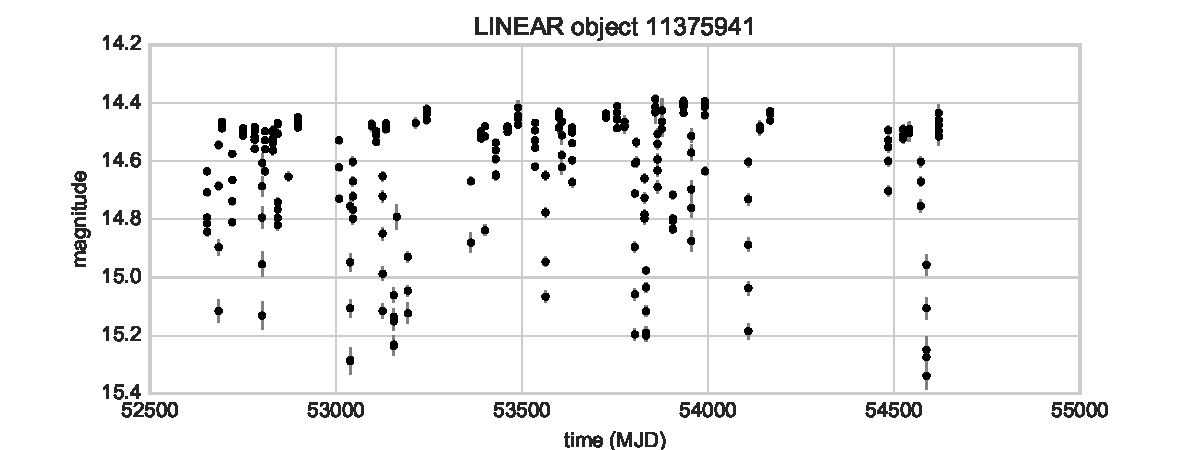
\includegraphics[width=\textwidth]{fig01_LINEAR_data}
\caption{Observed light curve from LINEAR object ID 11375941. Uncertainties
  are indicated by the gray errorbars on each point.
  \figlabel{LINEAR-data}
}
\end{figure}


\begin{figure}[ht]
\centering
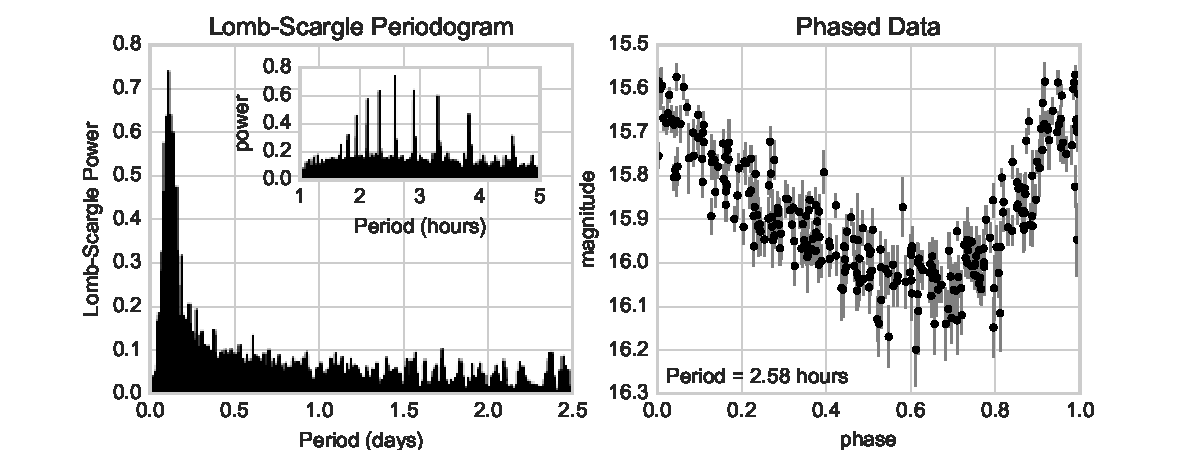
\includegraphics[width=\textwidth]{fig02_LINEAR_PSD}
\caption{{\it Left panel:} the Lomb-Scargle periodogram computed from the data
    shown in \fig{LINEAR-data}, with an inset detailing the region near the peak.
    {\it Right panel:} the input data in \fig{LINEAR-data}, folded over the
    detected 2.58-hour period to show the coherent periodic variability.
    For more discussion of this data, see \citep{LINEAR3}.
    \figlabel{LINEAR-power}
}
\end{figure}

The Lomb-Scargle periodogram \citep{Lomb76, Scargle82}
is a well-known algorithm for detecting periodicity
in unevenly-sampled time-series, particularly within the astronomy community.
For example, consider the data shown in \fig{LINEAR-data}.
This is an irregularly-sampled timeseries showing a single object from the
LINEAR survey \citep{LINEAR1, LINEAR3}, with magnitude measured 280 times over
the course of five and a half years\footnote{
  Python code to reproduce \fig{LINEAR-data}, as well as all other figures
  in this manuscript, is available at 
  \url{http://github.com/jakevdp/PracticalLombScargle/}}.

By eye, it is clear that the brightness of the object varies in time with a range spanning approximately 0.8 magnitudes, but what is not immediately clear is that this variation is periodic in time.
The Lomb-Scargle periodogram is a method that allows efficient computation of a Fourier-like power spectrum from such unevenly-sampled data, resulting in an intuitive means of determining the period of oscillation.

The left panel of \fig{LINEAR-power} shows the Lomb-Scargle periodogram computed for the data in \fig{LINEAR-data}.
Computing the Lomb-Scargle periodogram for the data gives us a measure of the
power as a function of period of oscillation (\fig{LINEAR-power}, left), from
which we can determine the period of oscillation of approximately 2.58 hours.
The right panel of \fig{LINEAR-power} shows a folded visualization of
the same data as \fig{LINEAR-data} -- i.e.{} plotted as a function of phase
rather than time.\footnote{
    The periodogram in \fig{LINEAR-power} was computed using
    {\tt astropy.stats.LombScargle}
    from the AstroPy project; see \url{http://astropy.org/}.
}

Often this is exactly how the Lomb-Scargle periodogram is presented: as a clean, well-defined procedure to detect the periodic component in an unevenly-sampled dataset.
In practice, however, there are a number of subtle issues that must be considered when applying a Lomb-Scargle analysis to real-world datasets, and I have found that these are rarely presented together at an introductory level.
Here are a few questions in particular that we might wish to ask about the results in \fig{LINEAR-power}:
\begin{enumerate}
  \item What is the source of the multiple peaks revealed by the Lomb-Scargle Periodogram?
  \item What is the Nyquist frequency for unevenly-sampled data?
  \item How should we choose the spacing of the frequency grid for our periodogram?
  \item What assumptions is the Lomb-Scargle periodogram making about the signal?
  \item How should we understand the uncertainty of the computed frequency?
\end{enumerate}
The answers to these sorts of questions are discussed in various textbooks and review papers, but I have not come across any single concise reference that gives a good intuition for how to think about such questions.
This paper seeks to fill that gap, and provide a practical, just-technical-enough guide to the effective use of the Lomb-Scargle method for periodic analysis.
This paper does not seek a complete or rigorous treatment of the mathematics involved, but rather seeks to develop the intuition of {\it how} to think about the issues involved.

The paper is organized as follows:
In \sect{continuous-fourier-transform}, we review the continous Fourier
transform and some of its useful properties, including defining the notion of
a power spectrum for measuring periodic content in a signal.
In \sect{window-functions}, we use these properties to understand how different
observation patterns (i.e. window functions) transform the power spectrum, and
discuss a conceptual understanding of the well-known Nyquist limit.
In \sect{non-uniform-sampling}, we consider non-uniformly sampled signals, and
show that the Nyquist limit for this case is quite different than what many
practitioners in the field seem to assume.
In \sect{schuster-to-lomb-scargle}, we discuss the Lomb-Scargle periodogram, a
modified version of the classical periodogram for unevenly-sampled data, as
well as the motivation behind these modifications.
In \sect{practical-considerations}, we discuss important practical
considerations for the use of the Lomb-Scargle periodogram, including
the choice of frequency grid and the various normalizations of the periodogram.
In \sect{uncertainties}, we discuss how to quantify uncertainties in periods
derived from the periodogram, including various notions of the
``False Alarm Probability''.
In \sect{generalizations}, we consider and critique some generalizations of
the Lomb-Scargle model, including multiterm periodograms and Bayesian
approaches.

All figures in this work were produced using Python, and in particular the
Numpy \citep{numpy},
Pandas \citep{pandas},
Astropy \citep{Astropy2013},
and Matplotlib \citep{matplotlib} packages.
Code to reproduce these figures is available in IPython notebooks at \url{http://github.com/jakevdp/PracticalLombScargle/}.

\section{Background: the Continuous Fourier Transform}
\sectlabel{continuous-fourier-transform}

In order to understand how we should interpret the Lomb-Scargle periodogram, we will first briefly step back and review the subject of Fourier analysis of continuous signals.
Consider a continuously-defined signal $g(t)$.
Its Fourier transform is given by the following integral:
\begin{equation}
    \hat{g}(f) \equiv \int_{-\infty}^\infty g(t) e^{-2\pi i f t} dt
    \eqlabel{FT-def}
\end{equation}
The inverse relationship is given by:
\begin{equation}
    g(t) \equiv \int_{-\infty}^\infty \hat{g}(f) e^{+2\pi i f t} df
    \eqlabel{IFT-def}
\end{equation}
For convenience we will also define the Fourier transform operator
$\mathcal{F}$, such that
\begin{eqnarray}
    \mathcal{F}\{g\} &=& \hat{g} \\
    \mathcal{F}^{-1}\{\hat{g}\} &=& g
\end{eqnarray}
As a further shorthand, we'll sometimes use a double arrow to denote a Fourier
pair; for example
\begin{equation}
  g(x) \Longleftrightarrow \hat{g}(f).
\end{equation}

\subsection{Properties of the Fourier Transform}

The continuous Fourier transform has a number of useful properties that we will make use of in our discussion.

\begin{description}
   \item[The Fourier transform is a linear operation.]
     That is, for any constant $A$ and any functions $f$ and $g$, we can write
     \begin{eqnarray}
       \mathcal{F}\{f(t) + g(t)\} &=& \mathcal{F}\{f(t)\} + \mathcal{F}\{g(t)\}\nonumber\\
       \mathcal{F}\{A f(t)\} &=& A\mathcal{F}\{f(t)\}
     \end{eqnarray}
     which follows from the linearity of the Fourier integral.

   \item[The Fourier transform of sinusoid with frequency $f_0$ is a sum of delta functions at $\pm f_0$.]
     Given the integral definition of the Dirac delta function, it is straightforward to show that
     \begin{equation}
       \mathcal{F}\{e^{2\pi f_0 t}\} = \delta(f - f_0).
       \eqlabel{delta-FT}
     \end{equation}
     Euler's formula shows how such a complex exponential
     can be expressed in terms of sines and cosines:
     \begin{equation}
       e^{2\pi f_0 t} = \cos(2\pi f_0 t) + i\sin(2\pi f_0 t).
       \eqlabel{Euler-formula}
     \end{equation}
     Using the linearity of the Fourier transform, we can take these identites
     and derive the following identities:
     \begin{eqnarray}
       \mathcal{F}\{\cos(2\pi f_0 t)\} &=& \frac{1}{2}\left[\delta(f - f_0) + \delta(f + f_0)\right]\nonumber\\
       \mathcal{F}\{\sin(2\pi f_0 t)\} &=& \frac{1}{2i}\left[\delta(f - f_0) - \delta(f + f_0)\right].
     \end{eqnarray}
     In other words, a sinusoidal signal with frequency $f_0$ has a Fourier transform consisting of a weighted sum of delta functions at $\pm f_0$.

   \item[A time-shift imparts a phase in the Fourier transform.]
     Given a well-behaved function $g(t)$ we can use a transformation of
     variables to derive the following identity:
     \begin{equation}
       \mathcal{F}\{g(t - t_0)\} = \mathcal{F}\{g(t)\} e^{-2\pi i ft_0}
     \end{equation}
     The key observation here is that the time-shift does not change the
     amplitude of the resulting transform, but only the phase.
\end{description}
These properties taken together make the Fourier transform quite useful for the study of periodic signals.
The linearity of the transform means that any signal made up of a sum of periodic components will have a Fourier transform consisting of a sum of delta functions at those frequencies: that is, the Fourier transform is a {\it direct} measure of the periodic content of a function.

Further, if we compute the squared amplitude of the resulting transform, we can both do away with complex components and remove the phase imparted by any time offsets; this squared amplitude is usually known as the {\it Power Spectrum}:
\begin{equation}
  \mathcal{P}\{g\} \equiv \left|\mathcal{F}\{g\}\right|^2
  \eqlabel{power-spectrum}
\end{equation}
The power spectrum of a function is a positive real-valued function of $f$ that quantifies the contribution of each frequency $f$ to the total signal.

\subsection{Some Useful Fourier Pairs}

\begin{figure}[ht]
\centering
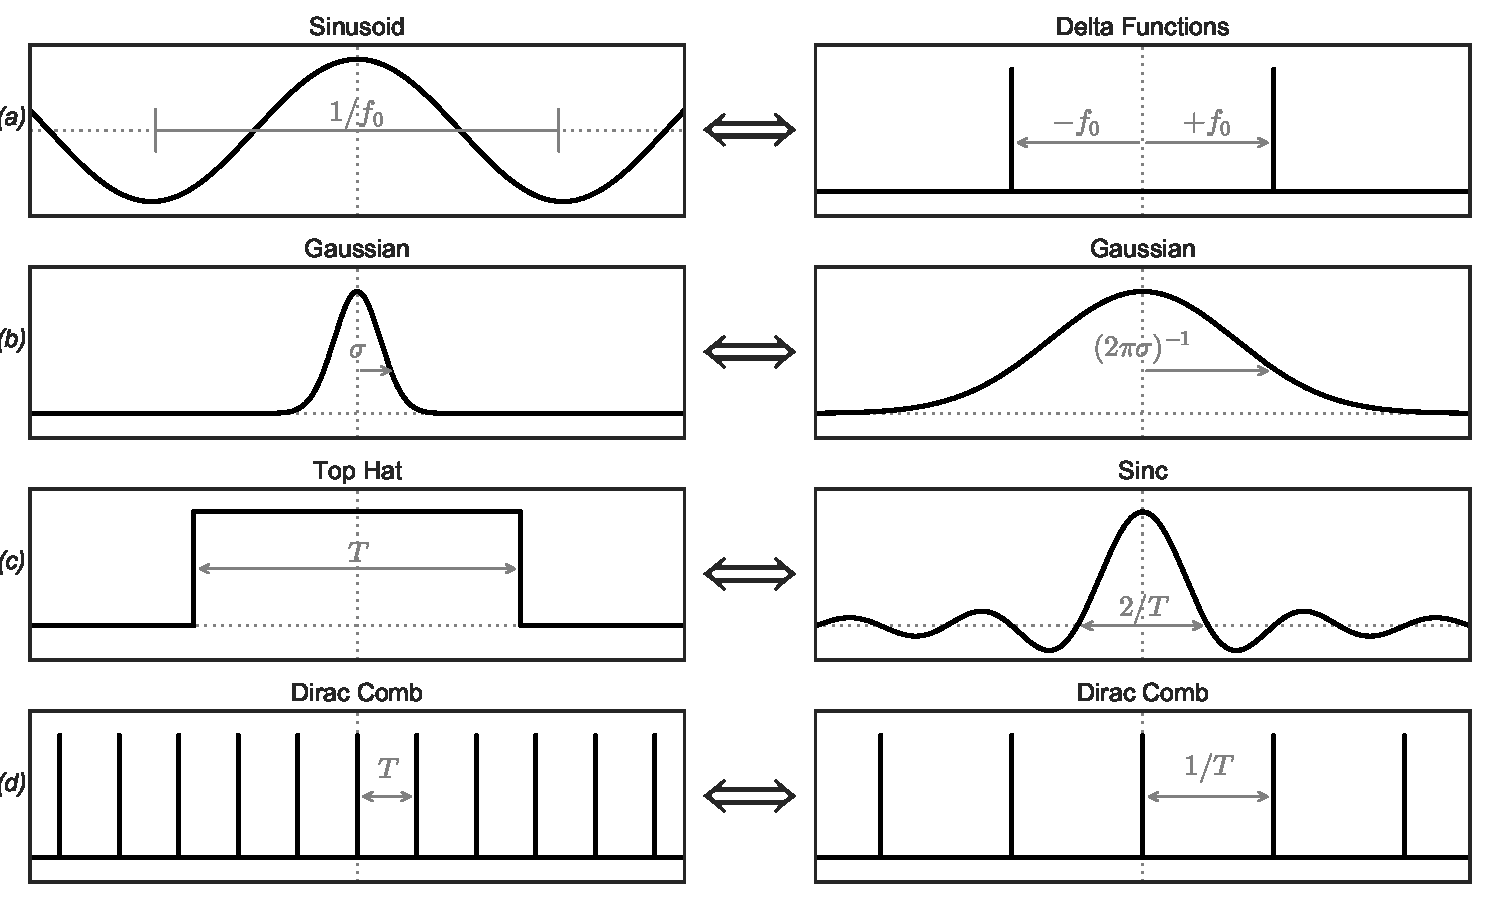
\includegraphics[width=\textwidth]{fig03_Fourier_pairs}
\caption{Visualization of important Fourier pairs.\figlabel{fourier-pairs}}
\end{figure}

We have already discussed that the Fourier transform of a complex exponential is a single delta function.
This is just one of many ``Fourier Pairs'' to keep in mind as we progress to understanding the Lomb-Scargle Periodogram.
We list a few more important pairs here (see \Fig{fourier-pairs} for a visual representation of the following pairs):


\begin{description}
  \item[The Fourier transform of a sinusoid is a pair of Delta functions.]
    (See \fig{fourier-pairs}{\it a})
    \begin{equation}
      \mathcal{F}\{\cos(2\pi f_0 t)\} = \frac{1}{2}\left[\delta(f-f_0) + \delta(f+f_0)\right]
    \end{equation}
    We saw this above, but repeat it here for completeness.

   \item[The Fourier transform of a Gaussian is a Gaussian.]
    (See \fig{fourier-pairs}{\it b})
     \begin{equation}
       \mathcal{F}\{{\rm N}(t; \sigma)\} = \frac{1}{\sqrt{2\pi\sigma^2}}{\rm N}\left(f;\frac{1}{2\pi\sigma}\right)
     \end{equation}
     The Gaussian function ${\rm N}(t, \sigma)$ is given by
     \begin{equation}
       {\rm N}(t; \sigma) \equiv \frac{1}{\sqrt{2\pi\sigma^2}}e^{-t^2/(2\sigma^2)}
     \end{equation}

  \item[The Fourier transform of a rectangular function is a sinc function.]
    (See \fig{fourier-pairs}{\it c})
    \begin{equation}
      \mathcal{F}\{\Pi_T(t)\} = \sinc(f T)
    \end{equation}
    The rectangular function, $\Pi(t)$, is a normalized symmetric function that
    is uniform within a range given by $T$, and zero elsewhere:
    \begin{equation}
      \Pi_T(t)  \equiv \left\{
      \begin{array}{ll}
        1 / T, & |t| \le T / 2 \\
        0,     & |t| > T / 2
      \end{array}
      \right.
    \end{equation}
    The sinc function is given by the standard definition:
    \begin{equation}
      \sinc(x) \equiv \frac{\sin(\pi x)}{\pi x}
    \end{equation}

  \item[The Fourier transform of a Dirac comb is a Dirac comb.]
    (See \fig{fourier-pairs}{\it d})
    \begin{equation}
      \mathcal{F}\{\III_T(t)\} = \frac{1}{T}\III_{1/T}(f)
    \end{equation}
    The Dirac comb, $\III_T(t)$, is an infinite sequence of Dirac delta functions placed at even intervals of size $T$:
    \begin{equation}
      \III_T(t) \equiv \sum_{n=-\infty}^\infty \delta(t - nT)
      \eqlabel{dirac-comb}
    \end{equation}
\end{description}
The key observation in each of these Fourier pairs is the reciprocity
of scales between a function and its Fourier transform:
that is, a function with a characteristic scale $T$ will in general
have a Fourier transform with characteristic scale of $1/T$.
This feature will turn out to be very important as we push further in
understanding the Lomb-Scargle Periodogram.


\subsection{The Convolution Theorem}

A final property of the Fourier transform that we will discuss here is its
ability to convert convolutions into point-wise products.
A convolution of two functions, usually denoted with a $\ast$, is defined
as follows:
\begin{equation}
  [f \ast g](t) = \int_{-\infty}^\infty f(\tau)g(t - \tau) d\tau
  \eqlabel{convolution-definition}
\end{equation}
From the definition, it is clear that a convolution amounts to ``sliding'' one
function past the other.
Such an operation is commonly used, for example, in smoothing a function,
as visualized in \Fig{convolution} for a rectangular smoothing window.

\begin{figure}[ht]
  \centering
  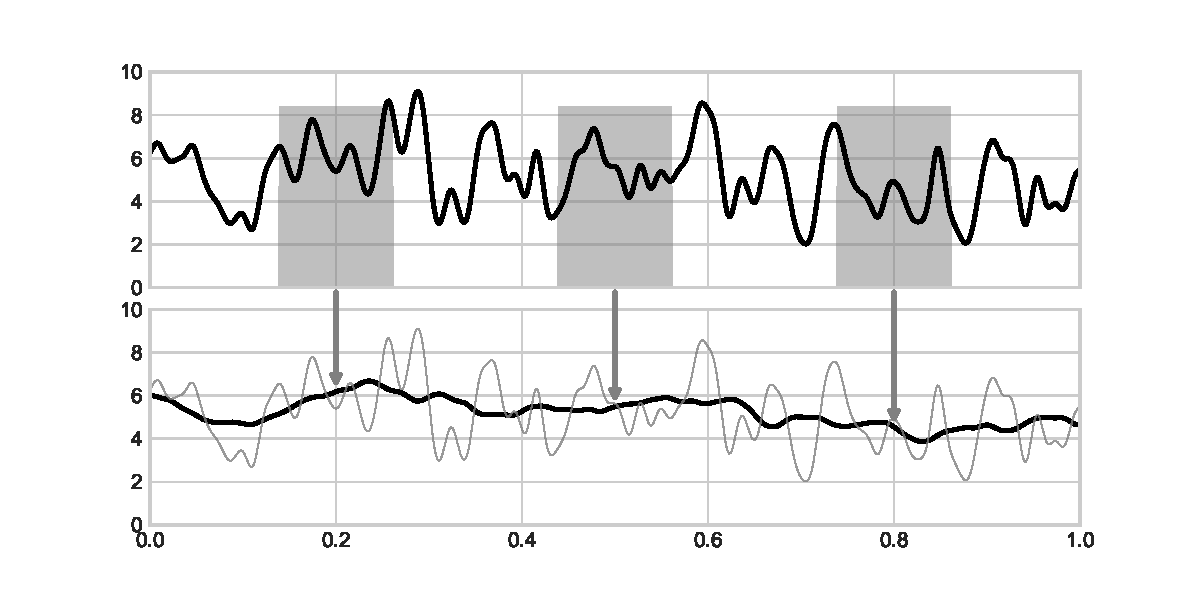
\includegraphics[width=\textwidth]{fig04_Convolution_Diagram}
  \caption{Visualization of a convolution between a continuous signal and a rectangular smoothing kernel.
    The normalized rectangular window function slides across the domain (upper panel),
    such that at each point the mean of the values within the window are
    used to compute the smoothed function (lower panel).
    \figlabel{convolution}}
\end{figure}

Given this definition of a convolution, it can be shown that the Fourier transform of a convolution is the point-wise product of the Fourier transforms:
\begin{equation}
  \mathcal{F}\{f \ast g\} = \mathcal{F}\{f\} \cdot \mathcal{F}\{g\}
  \eqlabel{convolution-theorem}
\end{equation}
In practice, this is a much more efficient means of computing the convolution
than to directly solve at each time $t$ the integral over $\tau$ that appears
in \eq{convolution-definition}.
This result in \eq{convolution-theorem} is known as the
{\it convolution theorem}, and is illustrated in \fig{convolution-theorem}.
\begin{figure}[ht]
  \centering
  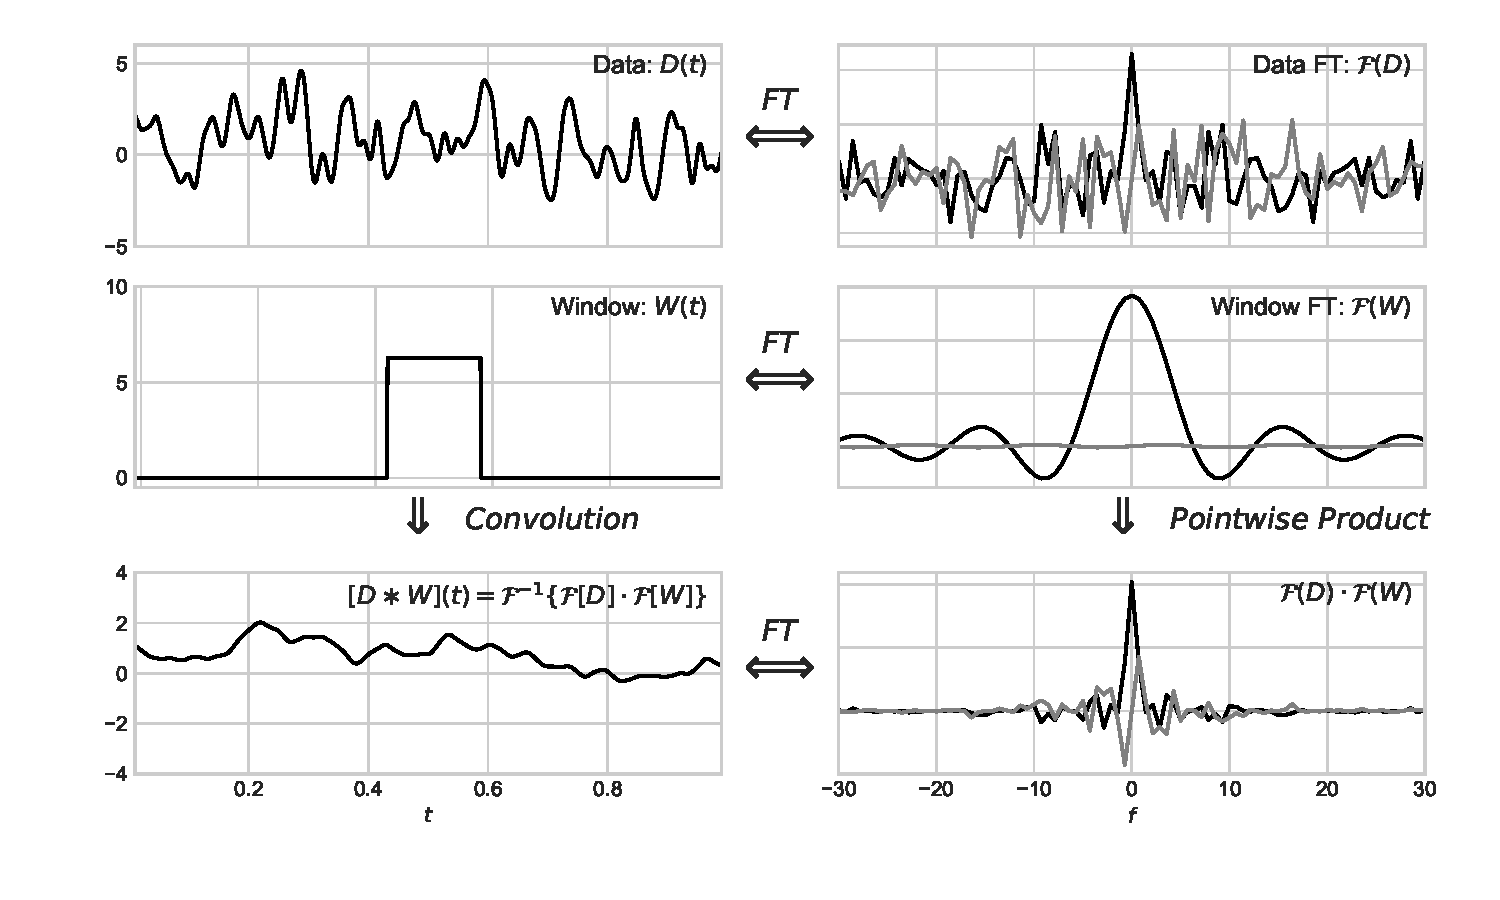
\includegraphics[width=\textwidth]{fig05_Convolution_Theorem}
  \caption{Visualization of the convolution theorem (\eq{convolution-theorem}).
    The key is that the Fourier transform of
    a convolution is the pointwise product of the two Fourier transforms.
    In the right panels, the black and gray lines represent the real and
    imaginary part of the transform, respectively.
    \figlabel{convolution-theorem}}
\end{figure}
When thinking about frequency components of time-domain measurements, this
property of the Fourier transform becomes essential, as we will see.

An important corrollary is that the Fourier transform of a product is a convolution of the two transforms:
\begin{equation}
  \mathcal{F}\{f \cdot g\} = \mathcal{F}\{f\} \ast \mathcal{F}\{g\}
  \eqlabel{convolution-theorem-inverse}
\end{equation}
We will explore the impact of this in the next section.

\section{Window Functions: From Idealized to Real-world signals}
\sectlabel{window-functions}

In a typical observational setting, we will be observing some small part of
a larger time-varying signal.
For example, if you have a very long signal that you measure for a finite
amount of time, your measurement is a point-wise product between the true
signal and a suitable rectangular function describing your measurement process.
If you have a continuous signal that you measure at regular intervals, your
measurement is a point-wise product between the true signal and an appropriate
Dirac comb describing your measurement process.
From what we learned about the convolution theorem in the previous section, it
is clear that {\it the measured Fourier transform will be the true transform
convolved with the transform of the obverving window}.
This has some interesting consequences, as we shall see.

\subsection{Effect of a Rectangular Window}

First, let's consider the case of observing a continuous periodic signal over
a limited span of time, as illustrated in \Fig{rectangular-window}.
Here we consider a periodic function made up of three frequency components, observed within a 10-unit time window.
The observed signal in this case can be thought of as a pointwise product of an infinite periodic signal, and a rectangular window function.
Using \eq{convolution-theorem-inverse}, we see that the Fourier transform of
this function is equivalent to the convolution of the Fourier transforms of each component, which are a set of delta functions and a sinc function, respectively.
For a purely periodic signal, this convolution has the effect of broadening the delta functions representing the signal, turning each of them into a shifted sinc function.
Because of the inverse relationship between the width of the window and the width of its transform (see \Fig{fourier-pairs}), it follows that a wider observing window leads to proportionally less spread in the Fourier transform of the observed function.

\begin{figure}[ht]
  \centering
  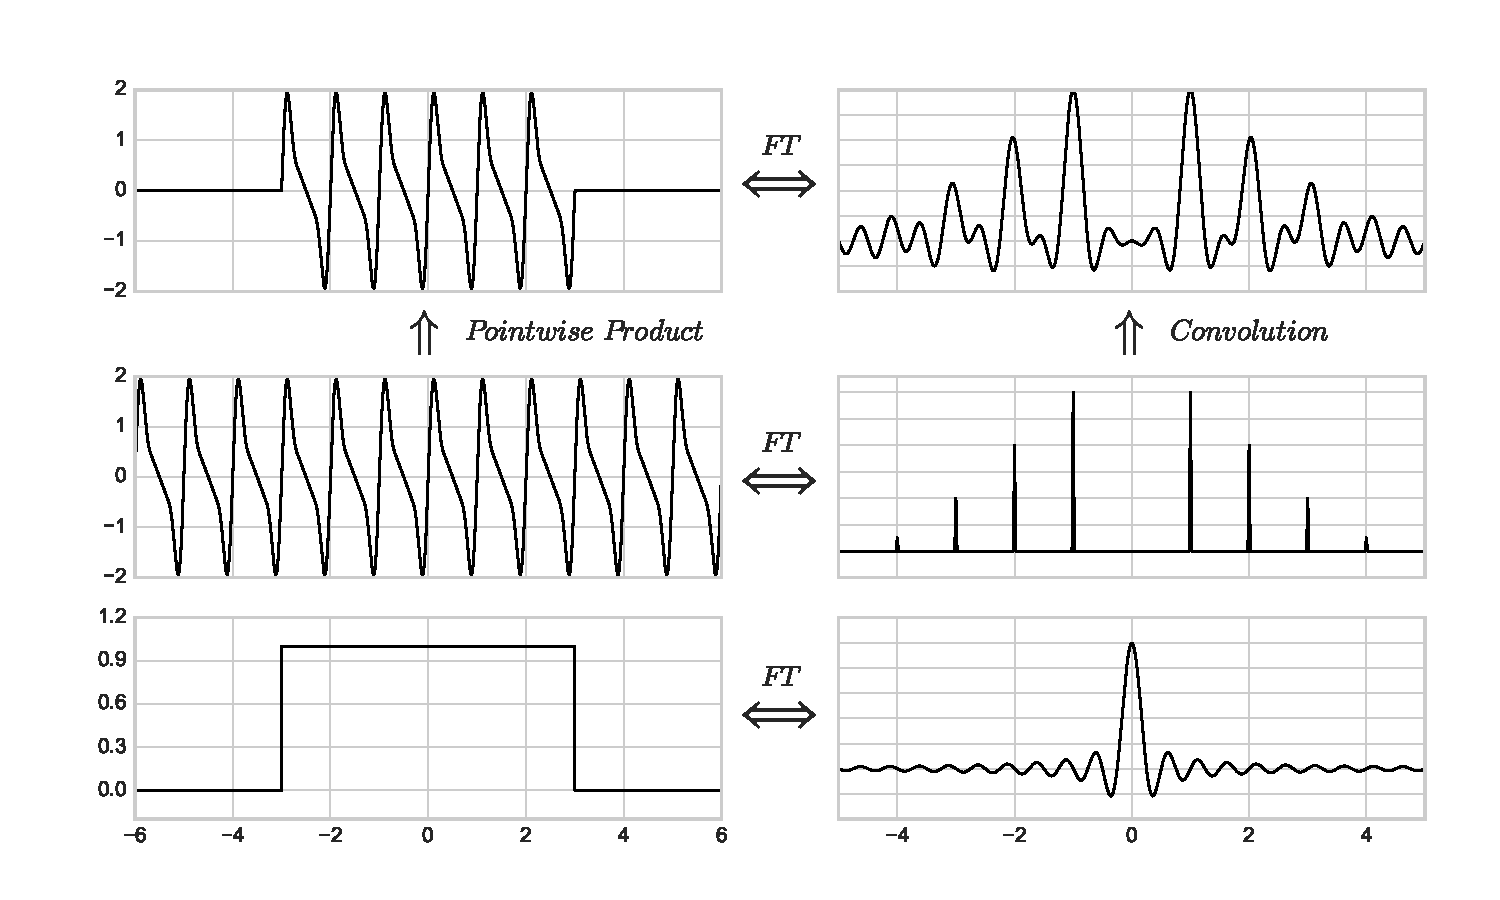
\includegraphics[width=\textwidth]{fig06_Rectangular_Window}
  \caption{Visualization of the effect on the Fourier transform of a
    rectangular observing window (i.e., a continuous signal observed in its
    entirety within a finite range of time). The observed Fourier
    transform is a convolution of the true transform (here a series of Delta
    functions) and the window transform (here a narrow sinc function).
    \figlabel{rectangular-window}}
\end{figure}

\subsection{The Dirac Comb and the Discrete Fourier Transform}
Another window function that commonly arises is when a continuous signal is
sampled instantaneously at regular intervals.
Such an observation is, in effect, a point-wise product between the true
underlying signal and a Dirac comb with the $T$ parameter matching the spacing
of the observations; this is illustrated in \fig{comb-window-1}.

\begin{figure}[ht]
  \centering
  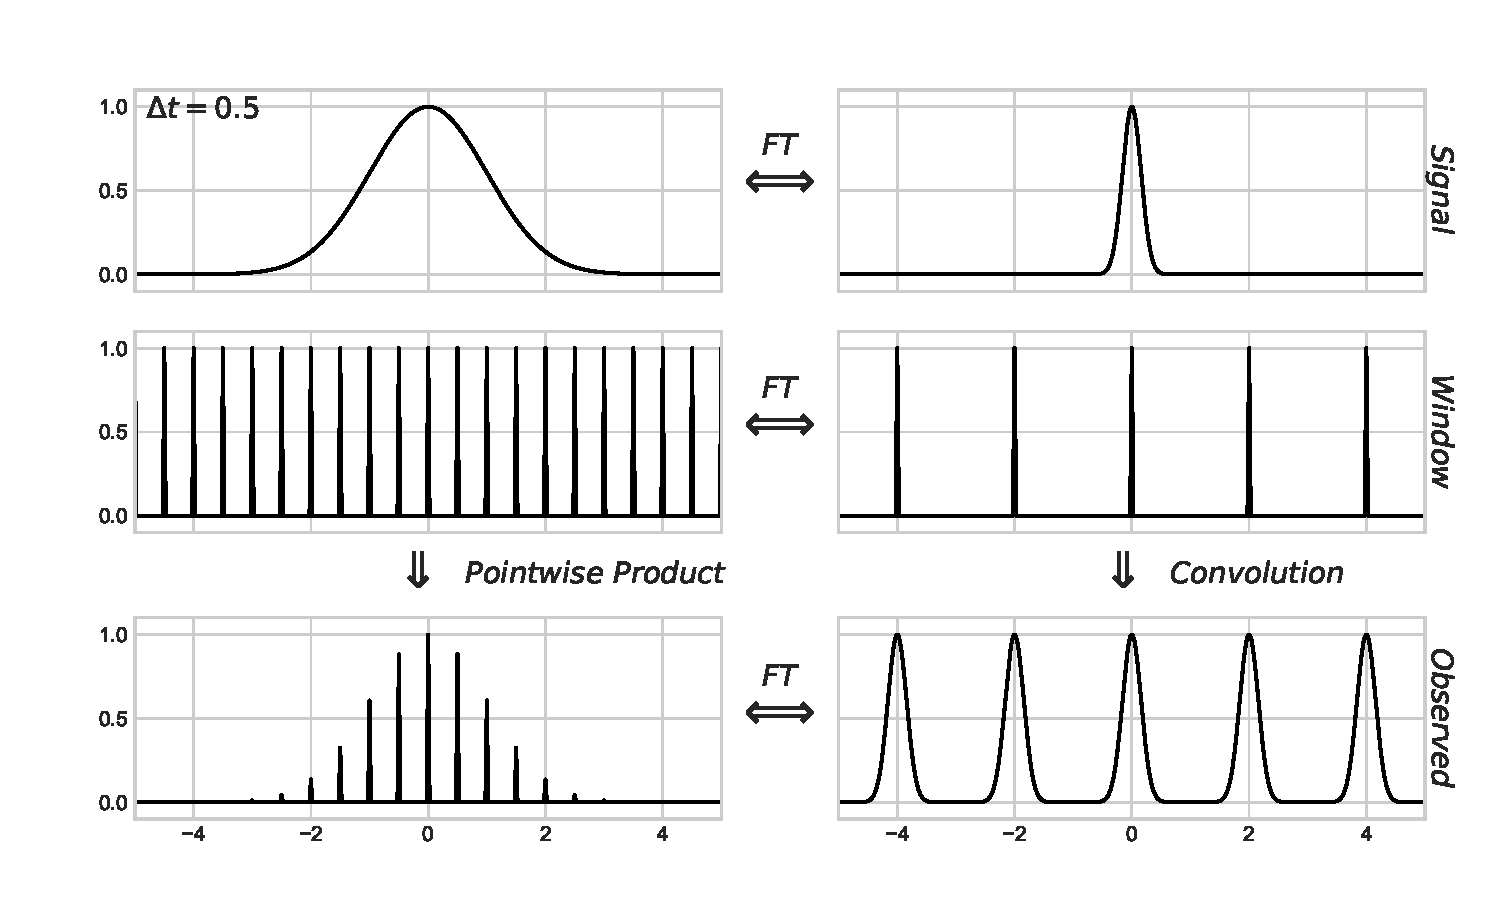
\includegraphics[width=\textwidth]{fig07_comb_window_1}
  \caption{Visualization of the effect on the Fourier transform of a
    Dirac Comb observing window (i.e., a long string of evenly-spaced
    discrete observations). The observed Fourier
    transform is a convolution of the true transform (here a localized
    Gaussian) and the window transform (here another Dirac comb).
    \figlabel{comb-window-1}}
\end{figure}

Interestingly, because the Fourier transform of a Dirac comb is another Dirac
comb, the effect of such an observing window is to create a long sequence
of aliases with a spacing of $1/T$.
With this in mind, we can be assured in this case that evaluating the
transform in the range $(2T)^{-1} \le f < (2T)^{-1}$ is sufficient to capture
all the available frequency information:
the signal outside that range is a sequence of identical aliases of
what lies in that range.
In fact, due to the nature of the aliasing, it is in fact sufficient to
compute the transform in {\it any} range of width $1/T$, and it is often
convenient to instead use the range $0 \le f < 1/T$.

\subsubsection{The Nyquist Limit}
\sectlabel{nyquist}

The example in \fig{comb-window-1} is somewhat of a best-case scenario, because
the true Fourier transform values lie entirely in a range of width $1/T$.
If we change the sampling rate so that this is no longer the case, we will
have a situation similar to that in \fig{comb-window-2}.
With a lower sampling rate, the signal transform no longer fits within the
frequency window, and the true Fourier transform {\it cannot be recovered}
from the observed transform.

This implies that if we have a regularly-sampled function with a sampling
rate of of $f_0 = 1/T$, we can only fully recover the freuqency information
if the signal is {\it band-limited} between frequencies $\pm f_0/2$.
This is one way to motivate the famous Nyquist sampling limit, which
approaches the question the other way around and says
that to fully represent the frequency content of a ``band-limited signal''
whose Fourier transform is zero outside the range $\pm B$,
we must sample the data with a rate of at least $2B$.

\begin{figure}[ht]
  \centering
  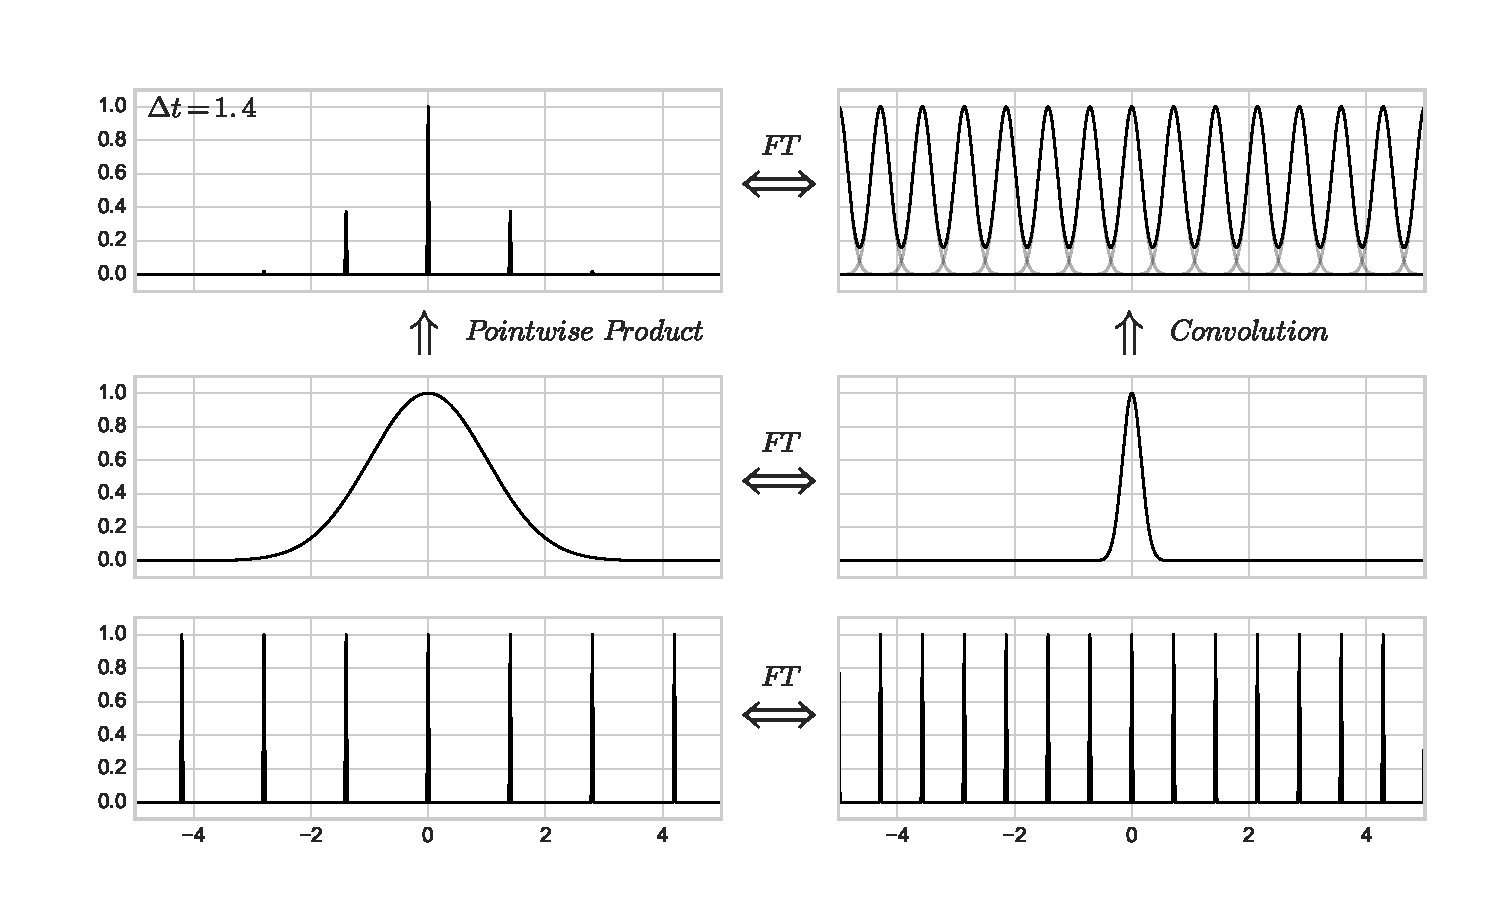
\includegraphics[width=\textwidth]{fig08_comb_window_2}
  \caption{Repeating the visualization from \fig{comb-window-1}, but here with
    a lower sampling rate. The result is that the Fourier transform of the
    window function (lower left) has spacing narrower than the Fourier transform
    of the signal (middle left), meaning the observed Fourier transform has
    aliasing of signals, such that not all frequency information can be
    recovered.
    \figlabel{comb-window-2}}
\end{figure}

\subsubsection{The Discrete Fourier Transform}
For regularly-spaced observations defined by a Dirac comb, the delta functions
serve to collapse the Fourier integral into a sum over periodic components.
Suppose we have a true (infinitely long and continuous) signal $g(t)$, but
we observe it only at a regular grid with spacing $T$. In this case, our
observed signal is $g_{obs} = g(t) \III_T(t)$ and its Fourier transform is
\begin{equation}
  \hat{g}_{obs}(f) = \sum_{n=-\infty}^\infty g(nT) e^{-2\pi i f n T},
\end{equation}
which follows directly from \eq{FT-def} and \eq{dirac-comb}.

In the real world, however, we will not have an infinite number of observations,
but rather a finite number of samples $N$.
We can choose the coordinate system appropriately and define
$g_n \equiv g(nT)$ to write
\begin{equation}
  \hat{g}_{obs}(f) = \sum_{n=0}^N g_n e^{-2\pi i f n T}
  \eqlabel{DFT-f}
\end{equation}
From the arguments around Nyquist aliasing, we know that the only relevant
frequency range is from $0 \le f \le 1/T$, and so we can define $N$
evenly-spaced frequencies with $\Delta f = 1 / (NT)$ covering this range.
Denoting the sampled transform as
$\hat{g}_k \equiv \hat{g}_{obs}(k\Delta f)$, we can write
\begin{equation}
  \hat{g}_k = \sum_{n=0}^N g_n e^{-2\pi i k n / N}
  \eqlabel{DFT}
\end{equation}
which you might recognize as the standard form of the discrete Fourier
transform.

You may have noticed we glossed over something here: the effect of switching
from an infinite number of samples to a finite number of samples.
In moving from $\hat{g}^{(T)}$ to $\hat{g}^{(N,T)}$, we have effectively applied
to our data a rectangular window function of width $NT$.
From the discussion accompanying \fig{rectangular-window}, we know what this does:
it gives us a Fourier transform convolved with a sinc function of width
$1 / (NT)$, resulting in the ``smearing'' of the Fourier transform signal
with this width.
Roughly speaking, then, any two Fourier transform values at frequencies within
$1/(NT)$ of each other will not be independent, and so we should space our
evaluations of the frequency with $\Delta f \ge 1/(NT)$.
Comparing to above, we see that this is {\it exactly the frequency spacing}
we arrived at from Nyquist-frequency arguments.

What this indicates is that the frequency spacing of the discrete Fourier
transform is optimal in terms of both the Nyquist sampling limit
{\it and} the effect of the finite observing window!
Now, this argument has admittedly been a bit hand-wavy, but there do exist
mathematically rigorous approaches to proving that the discrete Fourier
transform in \eq{DFT} captures all of the available frequency information
for a uniformly-sampled function $g_n$
\citep[see, e.g.][]{FoundationsOfSignalProcessing}.
Despite the semi-qualitative nature of our discussion,
I find it to be a helpful approach
in developing intuition regarding the relationship between the
continuous and discrete Fourier transforms.

\subsubsection{The Schuster Periodogram}

With the discrete Fourier transform defined in \eqs{DFT-f}{DFT}, we can
apply the definition of the Fourier power spectrum from \eq{power-spectrum}
to compute the {\it Schuster Periodogram}, first proposed by \citet{Schuster98}:
\begin{equation}
  P_S(f) = \frac{1}{N}\left|\sum_{n=1}^N g_n e^{-2\pi i f t_n}\right|^2
  \eqlabel{schuster-periodogram}
\end{equation}
Apart from the $1/N$ scaling, this is precisely the Fourier power defined
in \eq{power-spectrum} for the expression in \eq{DFT-f}, and it follows that
for a uniformly-sampled function $g_n$, the Schuster periodogram captures
all of the relevant frequency information present in the data.

\todo{Add simulated RR Lyrae data and show the Shuster periodogram}


\section{Non-uniform Sampling}
\sectlabel{non-uniform-sampling}

In the real world, particularly in fields like Astronomy where observations are
subject to interruptions from weather and diurnal cycles, the sampling rate
is generally far from uniform.
Using the same approach as we used to explore uniform sampling in the previous
section, we can now explore non-uniform sampling here.

In the general non-uniform case, we measure some signal at a set of $N$ times
which we will denote $\{t_n\}$.
Our observing window function in this case is still a sum of delta functions,
but at non-uniform locations.
Mathematically, the observing window will look like this:

\begin{equation}
W(t; \{t_n\}) = \sum_{n=1}^{N} \delta(t - t_n)
\end{equation}

Applying this window to our true underlying signal $g(t)$, we find an observed
signal of the form:

\begin{eqnarray}
  g_{obs}(t) &=& g(t) W(t; \{t_n\}) \nonumber\\
             &=& \sum_{n=1}^{N} g(t_n)\delta(t - t_n)
  \eqlabel{g-nonuniform}
\end{eqnarray}

Just as in the uniform case, the observed signal is a convolution of the true
signal transform and the window transform; unlike in the uniform case, the
window transform will generally {\it not} be a nice clean function.
\Fig{random-window} shows the effect on the Fourier transform of a
non-uniform observing cadence with a sampling rate identical to that
in \fig{comb-window-1}.

A few things stand-out in this figure. In particular, the Fourier transform of
the non-uniformly spaced delta functions looks like random noise, and in some
senses it is: the Fourier space representation reflects the frequency of
observations, and so non-structured spacing of observations will lead to
a non-structured Fourier representation of the window function.
This non-structured window transform, when convolved with the Fourier transform
of the true signal, results in an observed Fourier transform with the same
lack of useful structure.
Unlike the uniform result in \Fig{comb-window-1}, there is no direct aliasing
of the true signal, and no way to exactly recover any portion of the true
Fourier transform of this data.


\begin{figure}[ht]
  \centering
  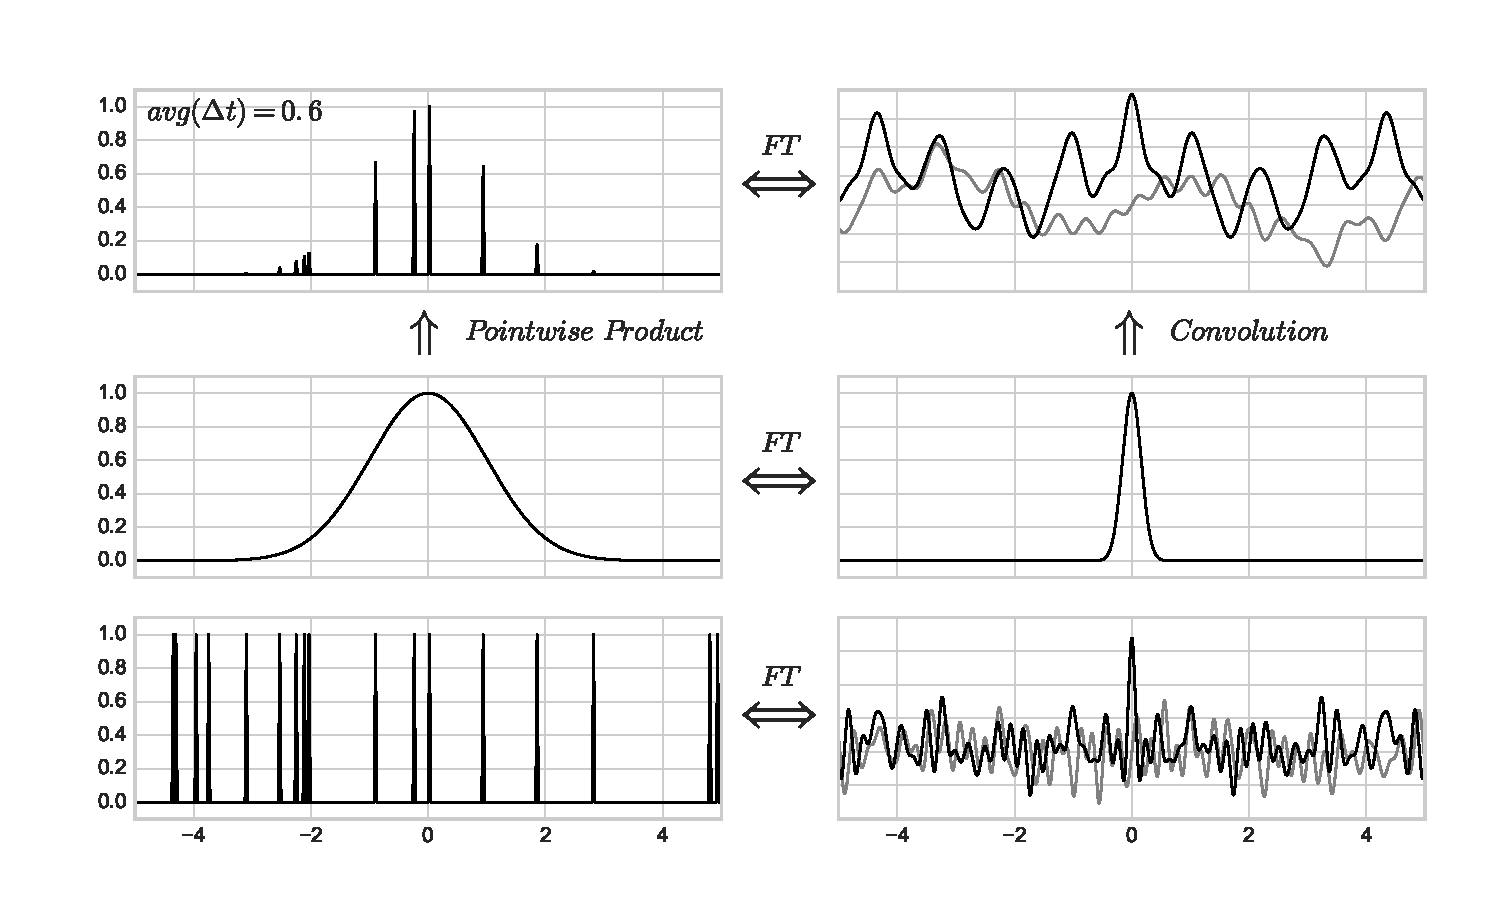
\includegraphics[width=\textwidth]{fig10_random_window}
  \caption{The effect of non-uniform sampling on the observed Fourier transform.
    These samples have the same average spacing as those in \fig{comb-window-1},
    but the lack of structure in observing window translates to a lack of
    structure in its transform, causing the observed transform to be ``noisy''.
    \figlabel{random-window}}
\end{figure}

One might hope that sampling the signal more densely might limit these problems,
and it does, but only to a degree.
\Fig{random-window-2} increases the density of observations by a factor of 10,
such that there are 200 total observations over the length-10 observing window.
The observed Fourier transform in this case is much more reflective of the
underlying signal, but still contains a degree of ``noise'' rooted in the
unstructured nature of the spacing between observations.


\begin{figure}[ht]
  \centering
  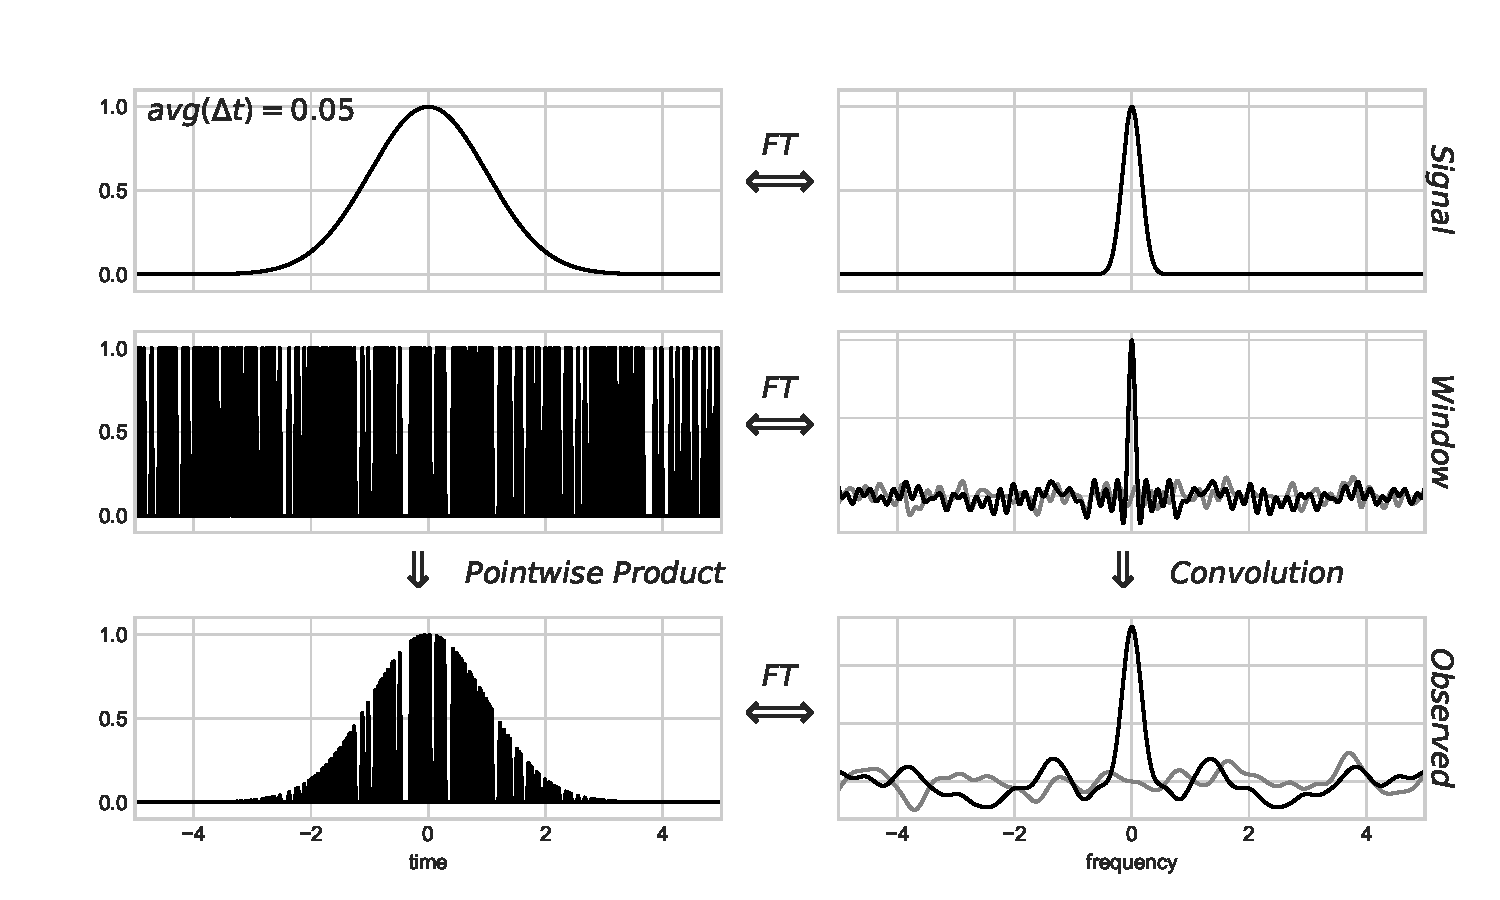
\includegraphics[width=\textwidth]{fig11_random_window_2}
  \caption{The effect of non-uniform sampling on the observed Fourier transform,
    with a factor of 10 more samples than \fig{random-window}.
    Even with very dense sampling of the function, the Fourier transform
    cannot be exactly recovered due to the 
    These samples have the same average spacing as those in \fig{comb-window-1},
    but the lack of structure in observing window translates to a lack of
    structure in its transform, causing the observed transform to be a
    ``noisy'' representation of the true transform
    \figlabel{random-window-2}}
\end{figure}

Since the observed transform is a well-defined convolution of the (unknown) true
transform and the (known) window transform, you might hope that we could
perform some sort of deconvolution operation to recover the result, but this
turns out not to be straightforward, as deconvolution (particularly in this
case where delta functions are involved) is an ill-posed problem without a
unique solution.

\subsection{Non-Uniform Periodogram}


From this non-uniform Fourier transform, it is straightforward to extend the
definition of the Schuster periodogram to the non-uniform case.
Plugging \eq{g-nonuniform} into the Fourier transform of \eq{FT-def}, in analogy to \eq{schuster-periodogram}, gives the following form of the power spectrum:
\begin{equation}
  P(f) = \frac{1}{N}\left|\sum_{n=1}^N g(t_n)e^{-2\pi i t_n} \right|^2
\end{equation}
Becuase it is derived from the Fourier transform of a non-uniformly sampled
function, this periodogram is subject to all the caveats mentioned here: in
particular, the periodogram measures the periodic content of the
{\it windowed signal} and thus reflects a convolution of the true signal
with a non-structured window function.
The resulting periodogram, then, can only be used as a qualitative approximation
of the true periodogram, and will only approach the true periodogram as the
number of observed samples gets very large.


\subsection{A Non-uniform Nyquist Limit?}
\sectlabel{pseudo-nyquist}

As we have seen in \sect{nyquist}, the Nyquist limit is a direct consequence
of the window function created by evenly-sampled data,
and uneven sampling destroys the symmetry that underlies its definition.
Nevertheless, the idea of the ``Nyquist frequency'' seems to have taken hold
in the scientific psyche to the extent that it's often mis-applied in areas
where it is utterly irrelevant.
For unevenly-sampled data, the ``Nyquist limit'' might or might not exist,
and even in cases where it does exist it tends to be far less relevant than
in the evenly-sampled case.

\subsubsection{Incorrect Limits in the Literature}

In the scientific literature it is quite common to come across various proposals
for a Nyquist-like or pseudo-Nyquist limit in the case of irregular sampling.
A few typical approaches include using the mean of the sampling intervals
\citep[e.g.][]{Scargle82, Horne86, NumRec},
the harmonic mean of the sampling intervals \citep[e.g.][]{Debosscher07},
or the minimum sample spacing \citep[e.g.][]{Percy86, Roberts87, Press89, Hilditch01}.
All of these are tempting criteria in that they recover the classical Nyquist 
frequency in the limit of evenly-spaced data.
Unfortunately, none of these approaches is correct: in general,
unevenly-sampled data can probe frequencies far larger than any of these
supposed limits (a fact that some of these citations do hint at
parenthetically).

As a simple example of where such logic fails,
consider the data from \fig{LINEAR-data}: though the mean sample
spacing is one observation every seven days, in \fig{LINEAR-power}
we were nevertheless able to quite clearly identify a period of 2.58 hours---
an order of magnitude shorter than the average-based pseudo-Nyquist limit
would indicate as possible.
For the data in \fig{LINEAR-data}, the minimum sample spacing is just under 10
seconds, but it would be irresponsible to claim that this single pair of
observations itself defines some limit beyond which frequency information is
unattainable.

\begin{figure}[ht]
  \centering
  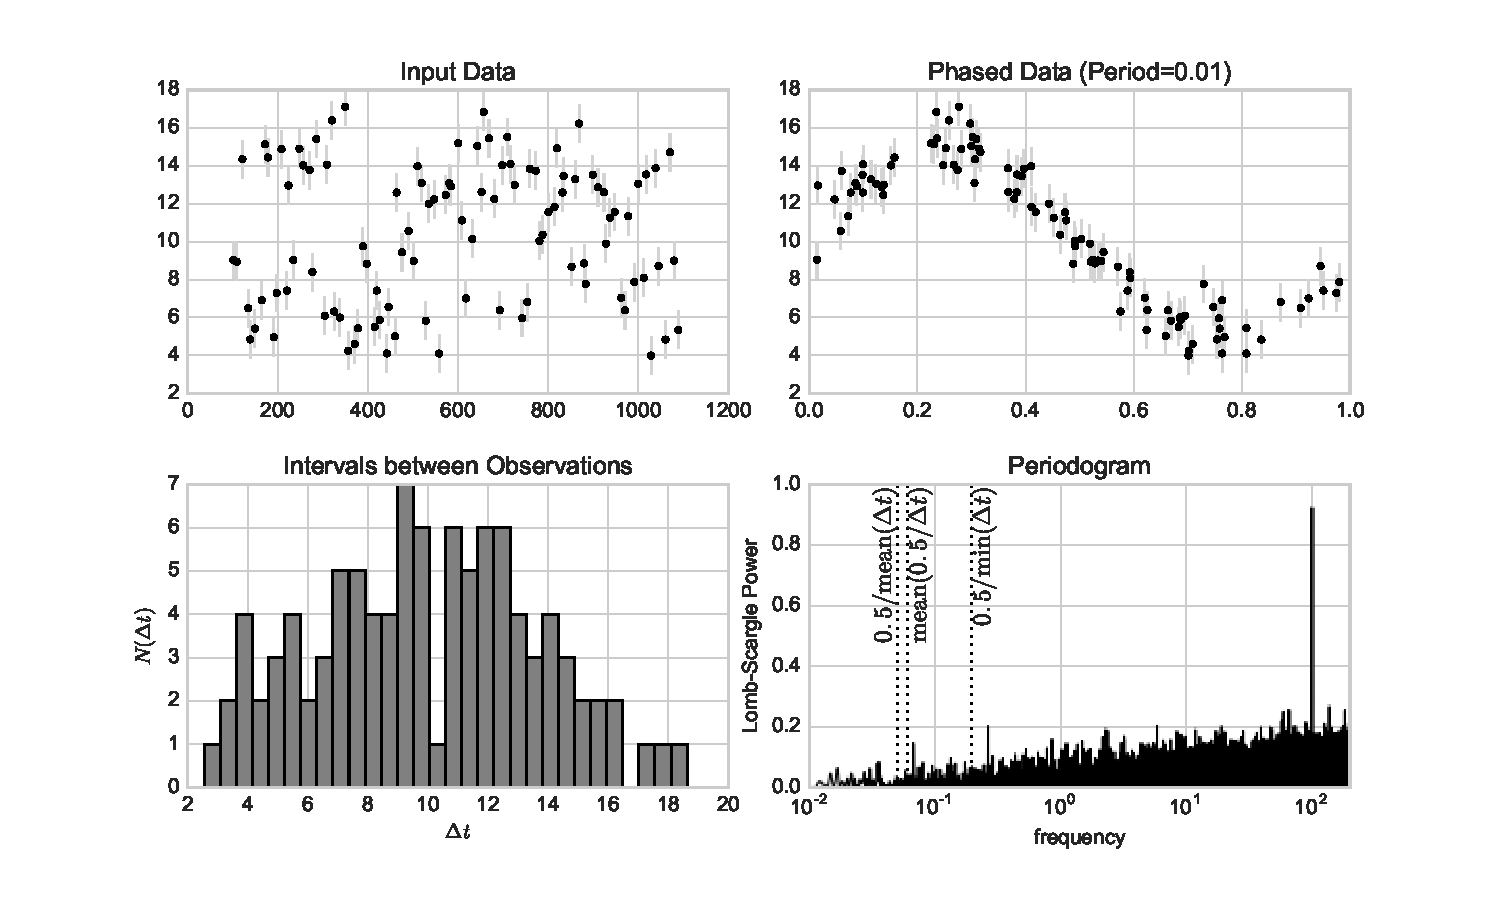
\includegraphics[width=\textwidth]{fig12_pseudo_nyquist}
  \caption{An example of data for which the various poorly-motivated
    ``pseudo-Nyquist'' approaches outlined in \sect{pseudo-nyquist} fail
    spectacularly. The upper panels show the data, a noisy sinusoid with
    a frequency of 100 (i.e. a period of 0.01).
    The lower left panel shows a histogram of spacings between observations:
    the minimum spacing is 2.55, meaning that the signal has
    {\it over 250 full cycles} between the closest pair of observations.
    Nevertheless, the periodogram (lower right) clearly identifies the correct
    period, though it's orders of magnitude larger than pseudo-Nyquist
    estimates based on average or minimum sampling rate.
    \figlabel{pseudo-nyquist}}
\end{figure}

As a more extreme example, consider the data shown in \fig{pseudo-nyquist}.
This consists of noisy samples from a sinusoid with a period of 0.01 units,
with sample spacings ranging between 2 and 18 units: needless to say, any
pseudo-Nyquist definition based on an average or minimum sample spacings
will be {\it far} smaller than the true frequency of 100; still, the
the Lomb-Scargle periodogram in the lower right panel shows quite cleanly
the true frequency.

\subsubsection{The Non-uniform Nyquist Limit}

While Nyquist arguments based on average or minimum sampling fail spectacularly,
there is a sense in which the Nyquist limit can be applied to unevenly-spaced
data. \citet{Eyer99} explores this issue in some detail, and in particular
proves the following:
\begin{quote}
Let $p$ be the largest value such that each $t_i$ can be written $t_i = t_0 + n_i p$, for integers $n_i$. The Nyquist Frequency then is $f_{Ny} = 1 / (2p)$.
\end{quote}
In other words, computing the Nyquist rate for unevenly-spaced data requires
finding some common factor, such that each spacing $\Delta t_i$ is {\it exactly}
an integer multiple of this factor.
This can be proven formally, but can be understood by thinking of such data as
a windowed version of uniformly sampled data with spacing $p$.
Such uniform data has a classical Nyquist limit of $1/(2p)$, and a window function applied to that data does not change that fact.

\Fig{nyquist-eyer99} shows an example of such a Nyquist frequency.
The data are non-uniformly sampled at times $t_i = n_i * p$, with $p=0.01$.
This results in a Nyquist frequency $f_{Ny} = 50$, and we see the expected
behavior beyond this frequency: the signal at $f > f_{Ny}$ consists of repeated
aliases of the signal at $f < f_{Ny}$.

\begin{figure}[ht]
  \centering
  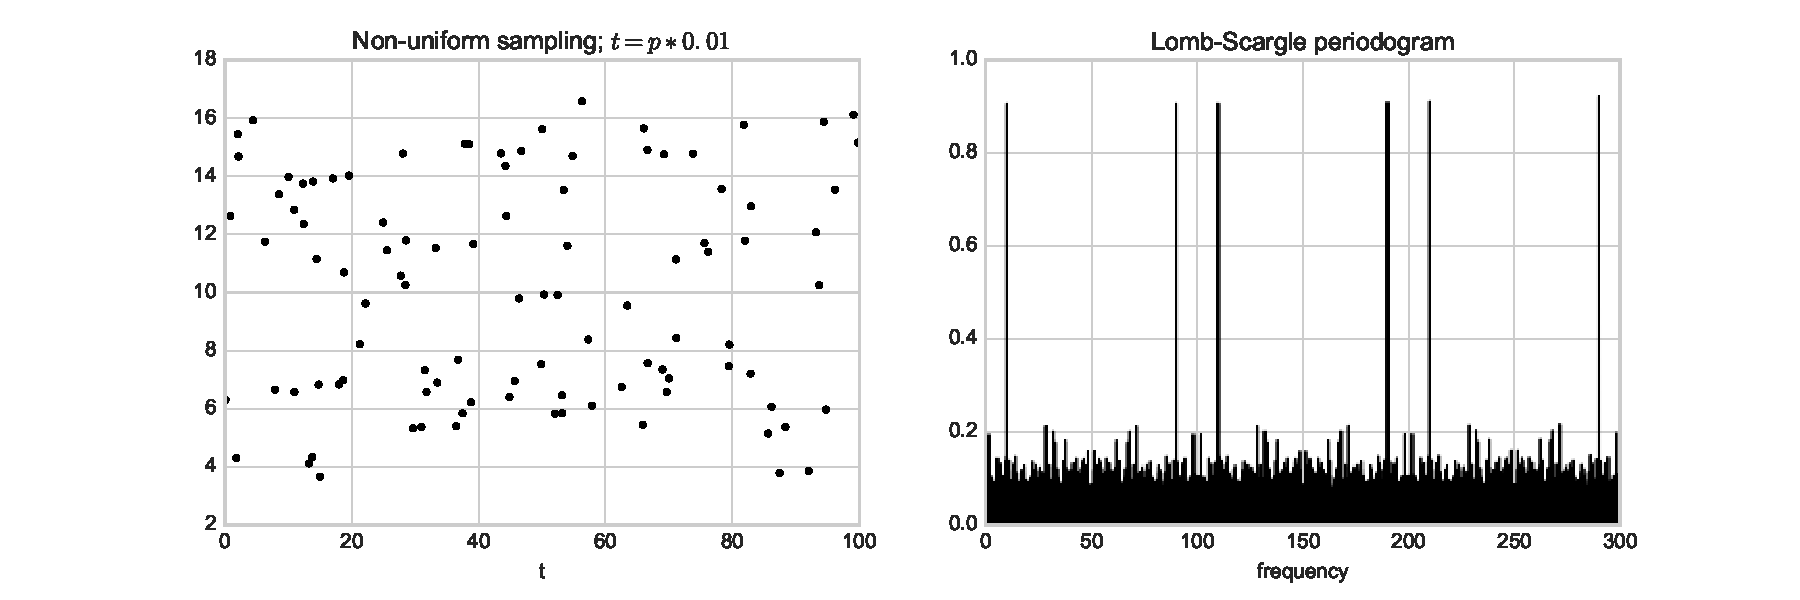
\includegraphics[width=\textwidth]{fig13_nyquist_eyer99}
  \caption{A visualization of the \citep{Eyer99} definition of the Nyquist
    frequency. Data are non-uniformly sampled at times $t_i = n_i p$, for
    integer $n_i$ and $p=0.01$.
    This results in a Nyquist frequency of $f_{Ny}= (2p)^{-1} = 50$:
    the periodogram outside the range $0 \le f < f_{Ny}$ is a series of
    perfect aliases of the signal within that range.
    \figlabel{nyquist-eyer99}}
\end{figure}

We should keep in mind one consequence of this Nyquist definition:
if you have any pair of observation spacings
whose ratio is irrational, {\it the Nyquist limit does not exist!}.
To realize this situation in practice, however, 
requires infinitely precise measurements of the
times $t_i$; more often in the real-world, the Nyquist frequency will be
defined by the precision of the time measurements.
That is, if times are recorded to $D$ decimal places, the Nyquist frequency
will be, at most
\begin{equation}
  f_{Ny} = \frac{1}{2} 10^D,
  \eqlabel{nonuniform-nyquist}
\end{equation}
as in \fig{nyquist-eyer99}.
In other words, absent other relevant patterns in the observations,
the Nyquist frequency for irregularly-sampled data is most
typically set by {\it the precision of the time measurements}.

\subsubsection{Limit due to Windowing}

In contexts where observations are not instantaneous, but rather consist of
short-duration integrations of a continuous signal, a qualitatively different
kind of frequency limit exists.
This is typical in, e.g., optical astronomy, where a single observation typically consists of an integration of observed flux over a finite duration $\delta t$.
As noted by \citet{ICVG2014}, this time-scale of integration represents another
kind of limiting frequency for irregularly-sampled data.
Such a situation means that the measurement is effectively a convolution of
the underlying signal with a rectangular window function of width $\delta t$,
in a manner analogous to \fig{convolution-theorem}.
By the convolution theorem, the observed transform will be a point-wise
product between the true transform and the transform of the window, which
will generally have a width proportional to $1/\delta t$.
This means that---absent other more constraining window effects---the
frequency limit is $f_{max} \propto 1/(2\delta t)$, with the constant of
proportionality dependent on the shape of the effective window describing
individual observations.

Keep in mind that the windowing limit $f_{max}$ is quite different than a
Nyquist limit: the Nyquist limit is the frequency beyond which all signal
is aliased into the Nyquist range; the windowing limit is the frequency
beyond which all signal is zero.

\subsection{Semi-structured Observing Windows}

We have seen that for uniform data, the perfect aliasing beyond the Nyquist
frequency is a direct consequence of the symmetry of the Dirac-comb window
function.
For non-uniform observations, such symmetry does not exist, but {\it structure}
in the observing window can lead to partial aliasing of signals in the
data \citep[see, e.g.][]{Deeming75}.


\begin{figure}[ht]
  \centering
  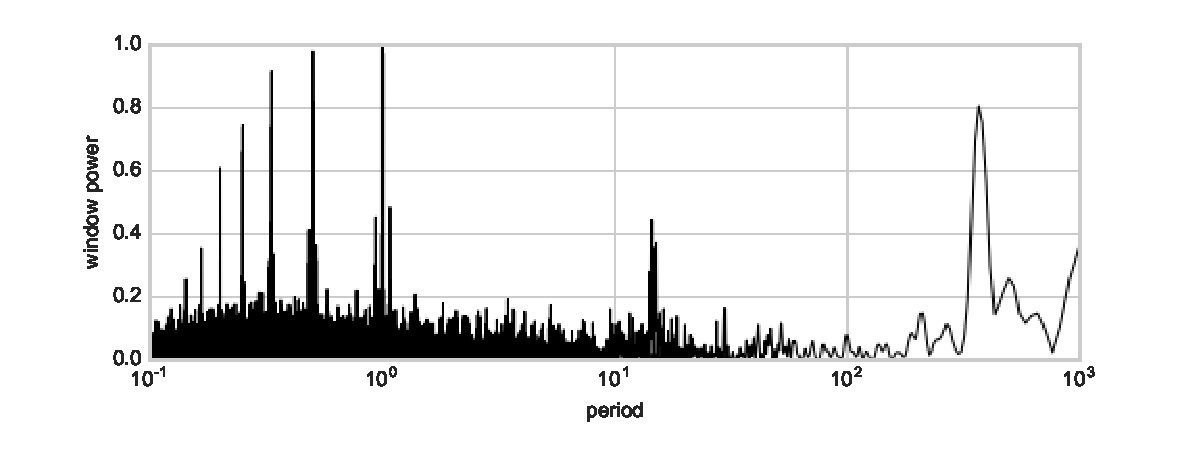
\includegraphics[width=\textwidth]{fig14_LINEAR_window}
  \caption{The power spectrum of the observing window for the data shown
    in \fig{LINEAR-data}. Notice the strong spike in power at a period of
    1 day, and related aliases at $1/n$ days for integer $n$.
    There is also a strong spike at $365$ days, and a noticeable spike at
    $\sim 14$ days. Each of these indicate time intervals that appear often
    in the data.
    \figlabel{LINEAR-window}}
\end{figure}

\subsubsection{A Ground-based Observing Window: LINEAR}

Let's again consider the data shown in \fig{LINEAR-data}. The window power
spectrum for this in \fig{LINEAR-window} shows some quite distinct features,
and these features have an intuitive interpretation.
Namely, if the window power shows a spike at a period of $p$ days, this means
that an observation at time $t_0$ is likely to be followed by another
observation near a time $t_0 + np$ for integer $n$.

Thus the strong spike at a period of 1 day indicate that observations are
taken near the same time of day: this is typical of a ground-based survey
which observes only at night.
The additional spikes at periods of $1/n$ days (for integer $n$) are aliases
of this same effect.

This window also shows a strong spike at a period of 1 year, indicating that
there was a strong seasonal pattern in the observations.
Finally, there is a noticeable spike at approximately 14 days that is likely
related to patterns in scheduling of observing runs.

Recall that a Fourier spectrum observed through a particular window will reflect
a convolution of the true spectrum and the window spectrum
(cf.\ \fig{random-window}), and so we would expect this structure to be
imprinted on the power spectrum measured from the data.


\begin{figure}[ht]
  \centering
  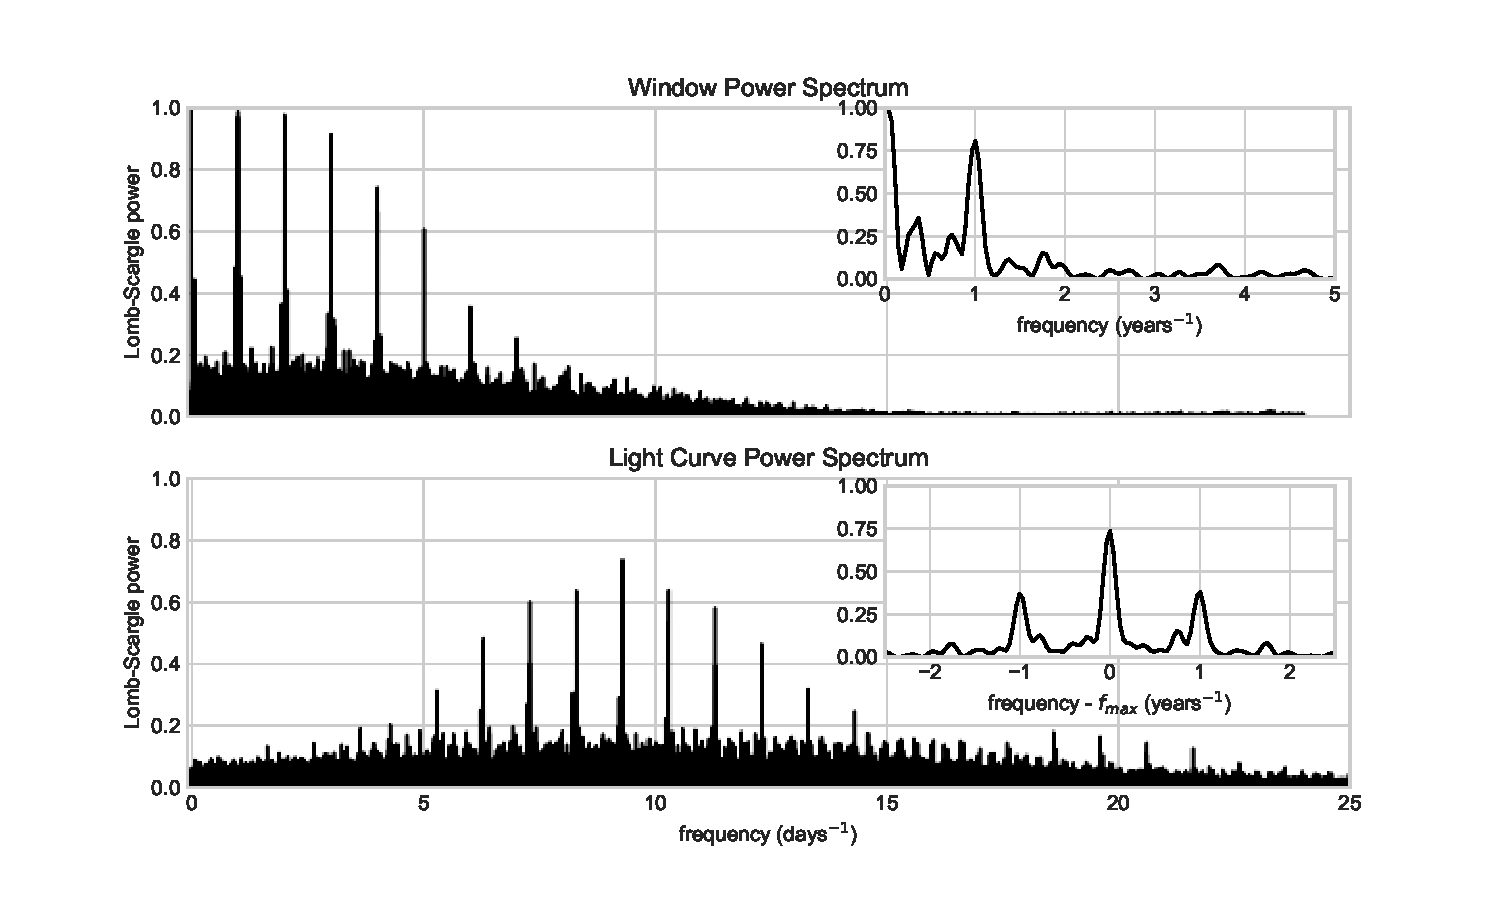
\includegraphics[width=\textwidth]{fig15_LINEAR_window_effect}
  \caption{The effect of the window function in \fig{LINEAR-window} on the
    power spectrum in \fig{LINEAR-power}.
    The top panel shows the window power spectrum, and the bottom panel shows
    the observed signal power spectrum.
    Both are plotted as a function of frequency (we earlier saw both of these
    as a function of period; see \fig{LINEAR-window} and \fig{LINEAR-power},
    respectively).
    Viewing these as a function of frequency makes it clear that the structure
    in the window function is imprinted on the observed spectrum: both the
    diurnal structure in the main panel, and the annual structure in the inset
    are apparent in the observed spectrum.
    \figlabel{LINEAR-window-effect}}
\end{figure}

This behavior is illustrated in \fig{LINEAR-window-effect}.
The upper panel shows the window power spectrum as a function of frequency, while lower panel shows the observed signal power spectrum as a function of frequency.
As noted in the discussion of \fig{LINEAR-window}, the window function shows a strong signal at frequencies corresponding to 1 day and 1 year; the latter can be seen in the inset plot.
The power at both these scales is clearly imprinted on the observed power spectrum, as shown in the lower panel and its inset.
This imperfect aliasing is similar to the perfect aliasing seen in regularly-sampled data at the Nyquist frequency; however, in this case the magnitude of the
aliased signal fades further from the frequency driving the signal.

\subsubsection{A Space-based Observing Window: Kepler}

\begin{figure}[ht]
  \centering
  \includegraphics[width=\textwidth]{fig16_kepler_data}
  \caption{An RR Lyrae variable observed by the Kepler project \citep[see][]{Kolenberg2010}.
    {\it upper left:} the 4083 observed fluxes over roughly three months.
    {\it upper right:} the window power spectrum, which is quite close to that of regularly-spaced data with a cadence of 29.4 minutes.
    {\it lower left:} the time between observations. other than missing measurements, the spacing between observations is nearly uniform. the lower panel gives a closer look at the majority of the spacings, which are not exactly the same but rather span a range of $\pm 50$ms around the main period observed in the window function.
    {\it lower right:} the data power spectrum, showing approximate aliasing and clearly indicating a peak near a period of 13.6 hours, along with higher-order components at multiples of this value.
    \figlabel{kepler-data}}
\end{figure}

Space-based missions often have quite different observing windows.
For example, the upper-left panel of \fig{kepler-data}
shows observations of an RR-Lyrae variable star from the Kepler survey,
measured over 4000 times over a period of three months,
with an irregular observing cadence of just under 30 minutes
 \citep[For deeper discussion of these observations, see][]{Kolenberg2010}.
The Kepler observations are very nearly uniformly-spaced, and this is reflected
in the window power spectrum, shown in the upper-right panel of
\fig{kepler-data}.
The window function is a series of very narrow evenly-spaced spikes,
reminiscent of the Dirac comb shown in \figs{comb-window-1}{comb-window-2},
which we used to motivate the idea of the Nyquist limit.
Thus, in this case we can treat $f_{Ny} = 0.5/29.4$ minutes$^{-1}$ as the
effective Nyquist limit for the data, though aliasing is imperfect due to
the uneven spacing of samples, shown in the lower-left panels of
\fig{kepler-data}.

The lower-right panel of \fig{kepler-data} shows the power spectrum of the
observations, with gray shading indicating the ``Aliased'' region of the
spectrum.
The period of 13.6 hours is strongly apparent, along with smaller spikes at
integer multiples of this frequency that indicate higher-order periodic
components in the signal.

The window functions for ground-based and space-based observations, reflected
by LINEAR data in \fig{LINEAR-window-effect} and Kepler data in
\fig{kepler-data}, are quite different, but in both cases essential features
of the observed power spectra can be understood by recognizing it reflects
not the power spectrum of the underlying signal, but a power specrtrum from
the convolution of the true signal transform and the Fourier transform of
the window function.
For another example of this type of observing window analysis, see
\citep{Deeming75}


\section{From Schuster to Lomb-Scargle}
\sectlabel{schuster-to-lomb-scargle}

Up until now, we've been mainly discussing the direct extension of the Schuster
periodogram in \eq{schuster-periodogram} to non-uniform data.
Returning to this definition, we can rewrite the expression in a more
suggestive way:
\begin{eqnarray}
  P(f)
  &=& \frac{1}{N}\left|\sum_{n=1}^N g(t_n)e^{-2\pi i t_n} \right|^2 \nonumber\\
  &=& \frac{1}{N}\left[
    \left(\sum_n g_n \cos(2\pi f t_n)\right)^2
    + \left(\sum_n g_n \sin(2\pi f t_n)\right)^2
    \right]
  \eqlabel{classical-periodogram}
\end{eqnarray}
Although this form of the non-uniform periodogram can be useful for identifying
periodic signals, its statistical properties are not as straightforward as in
the uniform case.
In this case, when we say an estimator with ``good statistical properties'',
we mean that when it is applied to data with straightforward, uncorrelated
noise, the result is a periodogram estimate in which the noise is also
straightforward and uncorrelated.

\citet{Scargle82} showed that while the classical periodogram of
\eq{classical-periodogram} has these desireable statistical properties
in the case of uniform sampling, this does not hold for
\eq{classical-periodogram} when the sampling becomes non-uniform.
To address this, he considered a generalized form of the periodogram,
\begin{equation}
  P(f) = \frac{A^2}{2}\left(\sum_n g_n \cos(2\pi f [t_n-\tau])\right)^2
       + \frac{B^2}{2} \left(\sum_n g_n \sin(2\pi f [t_n-\tau])\right)^2,
\end{equation}
where $A$ and $B$ are arbitrary functions of the frequency $f$ and
observing times $\{t_i\}$ (but not the values $\{g_n\}$, and showed
that you can choose one particular form of $A$ and $B$ such that
\begin{enumerate}
  \item The periodogram reduces to the classical form in the case of equally-spaced data,
  \item The periodogram has desireable statistical properties, in the sense discussed above,
  \item The periodogram is insensitive to global time-shifts in the data.
\end{enumerate}
The values of $A$ and $B$ leading to these properties lead to the following
modification of the classical expression for the periodogram:
\begin{eqnarray}
  P(f) =
  \frac{1}{2} \Bigg\{ &
  \bigg(\sum_n g_n \cos(2\pi f [t_n-\tau])\bigg)^2 \bigg/
  \sum_n \cos^2(2\pi f [t_n-\tau]) &\nonumber\\
  & + ~ \bigg(\sum_n g_n \sin(2\pi f [t_n-\tau])\bigg)^2 \bigg/
  \sum_n \sin^2(2\pi f [t_n-\tau]) & \Bigg\}
  \eqlabel{lomb-scargle-periodogram}
\end{eqnarray}
where $\tau$ is specified for each $f$ to ensure time-shift invariance:
\begin{equation}
  \tau = \frac{1}{4\pi f}\tan^{-1}\Bigg(
  \frac{\sum_n \sin(4\pi f t_n)}{\sum_n \cos(4\pi f t_n)}\Bigg).
  \eqlabel{tau-def}
\end{equation}
This modified periodogram differs from the classical periodogram only to
the extent that the denominators $\sum_n \sin^2(2\pi f t_n)$ and
$\sum_n \cos^2(2\pi f t_n)$ differ from $N/2$, which is the expected value of
each of these quantities in the limit of complete phase sampling at each
frequency.
Thus, in many cases of interest the Lomb-Scargle periodogram only differs
slightly from the classical/Schuster periodogram; an example of this is seen
in \fig{ls-comparison}.

\begin{figure}[ht]
  \centering
  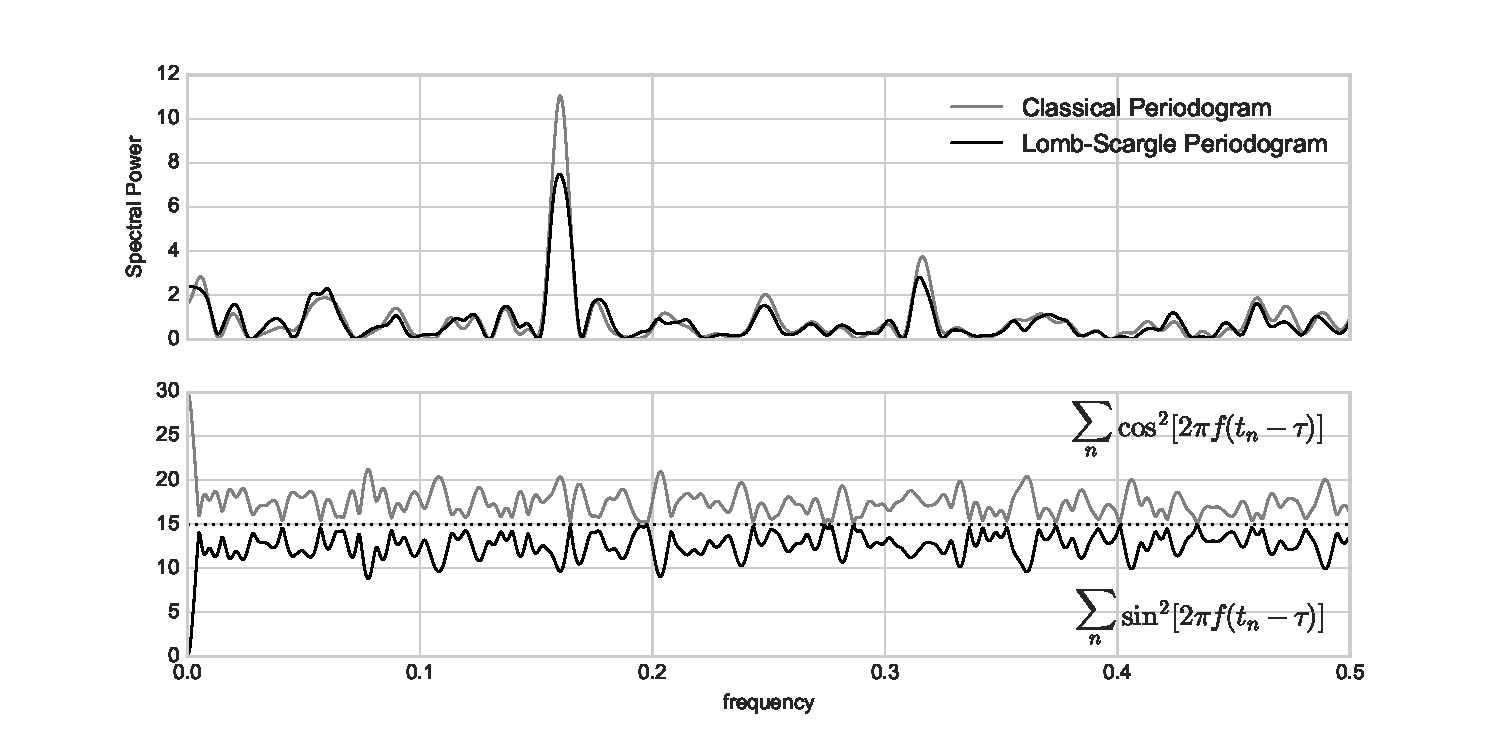
\includegraphics[width=\textwidth]{fig17_ls_comparison}
  \caption{{\it upper panel:} A comparison of the Classical periodogram
    (\eq{classical-periodogram}) and the Lomb-Scargle periodogram
    (\eq{lomb-scargle-periodogram}) for 30 noisy points drawn from a sinusoid.
    Though the two periodogram estimates differ quantitatively, the essential
    qualitative features---namely the position of significant peaks---generally
    remain the same.
    {\it lower panel:} the values of the denominators in
    \eq{lomb-scargle-periodogram}.
    The difference between the Lomb-Scargle periodogram and the classical
    periodogram stems from the difference between these quantities
    and $N/2 = 15$ (the dotted line).
    \figlabel{ls-comparison}}
\end{figure}

A remarkable feature of Scargle's modified periodogram is that it is
{\it identical} to the result
obtained by fitting a model consisting of a simple sinusoid to the data at
each frequency $f$ and
constructing a ``periodogram'' from the $\chi^2$ goodness-of-fit at each
frequency--an estimator which was considered in some depth by \citet{Lomb76}.
In this view, the $\tau$ shift defined in \eq{tau-def} serves to orthogonalize
the normal equations used in the least squares analysis.

Partly due to the deep connection between Fourier analysis and least-squares
analysis, the modified periodogram in \eq{lomb-scargle-periodogram}
has since become commonly referred to as the {\it Lomb-Scargle Periodogram}.

Because of this similarity between the classical and Lomb-Scargle periodograms,
our discussion of windowing effects applies---at least qualitatively---to
results computed with the Lomb-Scargle periodogram.
In particular, reasoning about the effect of window functions on the observed
Lomb-Scargle power spectrum remains useful even if it is true in only a
qualitative sense.


\section{Least-Squares Extensions to Lomb-Scargle}
\sectlabel{lomb-scargle-extensions}

\begin{figure}[ht]
  \centering
  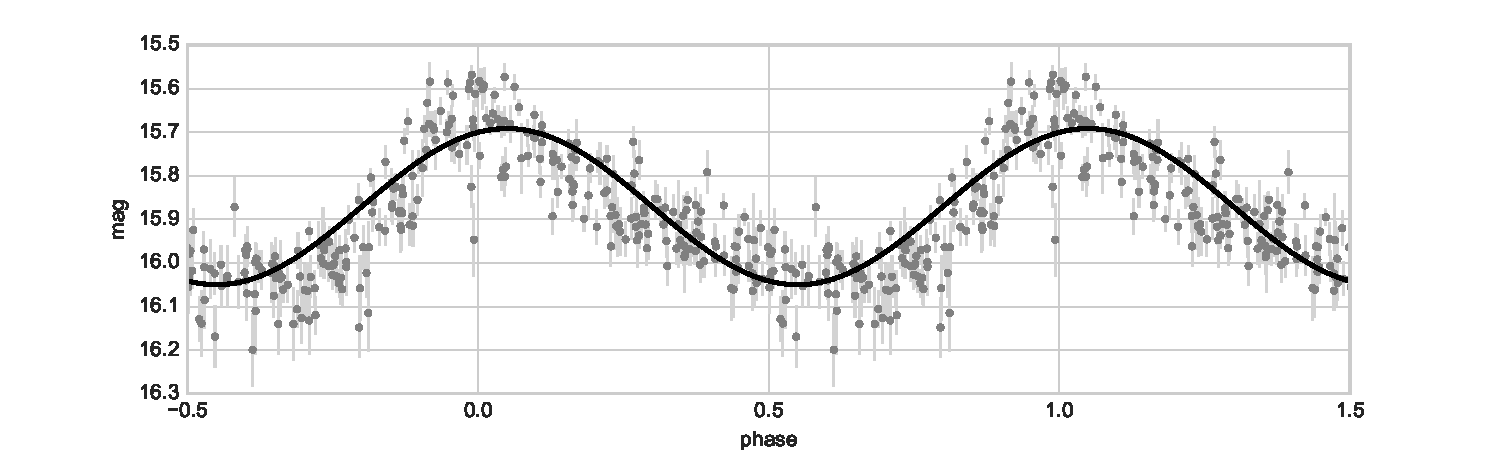
\includegraphics[width=\textwidth]{fig18_ls_model}
  \caption{The sinusoidal model implied by the Lomb-Scargle periodogram for
    the LINEAR data seen in \fig{LINEAR-data}.
    Although a sinusoid does not perfectly fit the data, it is close enough
    that it serves to find the correct period without a problem.
    \figlabel{ls-model}}
\end{figure}

The equivalence of the Fourier interpretation and least squares interpretation of the Lomb-Scargle periodogram allows for some interesting and useful extensions to the periodogram.
In the least squares interpretation of the periodogram, a sinusoidal model is proposed at each candidate frequency $f$:
\begin{equation}
  y_{model}(t;f) = A_f \sin(2 \pi f (t - \phi_f))
\end{equation}
where the amplitude $A_f$ and phase $\phi_f$ can vary as a function of frequency.
This is fit to the data in the standard least-squares sense, by constructing
the $\chi^2$ statistic at each frequency:
\begin{equation}
  \chi^2(f) \equiv \sum_n \big(y_n - y_{model}(t_n;f)\big)^2
  \eqlabel{chi2-simple}
\end{equation}
We can find the ``best'' model $\hat{y}(t;f)$ by minimizing $\chi^2(f)$ at
each freuqnecy with respect to $A_f$ and $\phi_f$;
we will denote this minimum value as $\hat{\chi}^2(f)$.
\citet{Scargle82} showed that with this setup, the Lomb-Scargle
periodogram from \eq{lomb-scargle-periodogram} can be equivalently written:
\begin{equation}
  P(f) = \frac{N}{2}\big[\hat{\chi}^2_0 - \hat{\chi}^2(f)\big]
  \eqlabel{lomb-scargle-chi2}
\end{equation}
where $\hat{\chi}^2_0$ is the reference model that assumes no variation in the data.
The key realization here is that the Lomb-Scargle periodogram essentially
{\it assumes a sinusoidal model} for the data; this is visualized in
\fig{ls-model} for the data we had seen in \fig{LINEAR-data}.
This immediately begs the question: can we compute a ``periodogram'' based
on more general forms of $y(t;f)$ to more effectively fit the data?


\subsection{Observational Noise}
\label{extensions-observational-noise}
Perhaps the most immediately obvious modification of the periodogram is to
change not the form of the model $y_{model}$, but the $\chi^2$ statistic itself
to account for observational errors in the data.
If there are Gaussian errors $\sigma_n$ on each observed $y_n$, we can re-write \eq{chi2-simple} in the following (standard) way:
\begin{equation}
  \chi^2(f) \equiv \sum_n \left(\frac{y_n - y_{model}(t_n;f)}{\sigma_n}\right)^2
  \eqlabel{chi2-with-errors}
\end{equation}
The periodogram constructed from this $\chi^2$ definition will more accurately
reflect the spectral power of noisy observations.
The effect of this modification on \eq{lomb-scargle-periodogram} is the addition
of a multiplicative weight $1/\sigma_n$ within each of the summations.
Early versions of this sort of modification appear in \citet{Gilliland87}
and \citet{Irwin89}; \citet{Zechmeister09} showed that such a modification
does not change the desirable statistical properties of the periodogram.


\subsection{Data Centering and the Floating Mean Periodogram}
\sectlabel{centering-data}

\begin{figure}[ht]
  \centering
  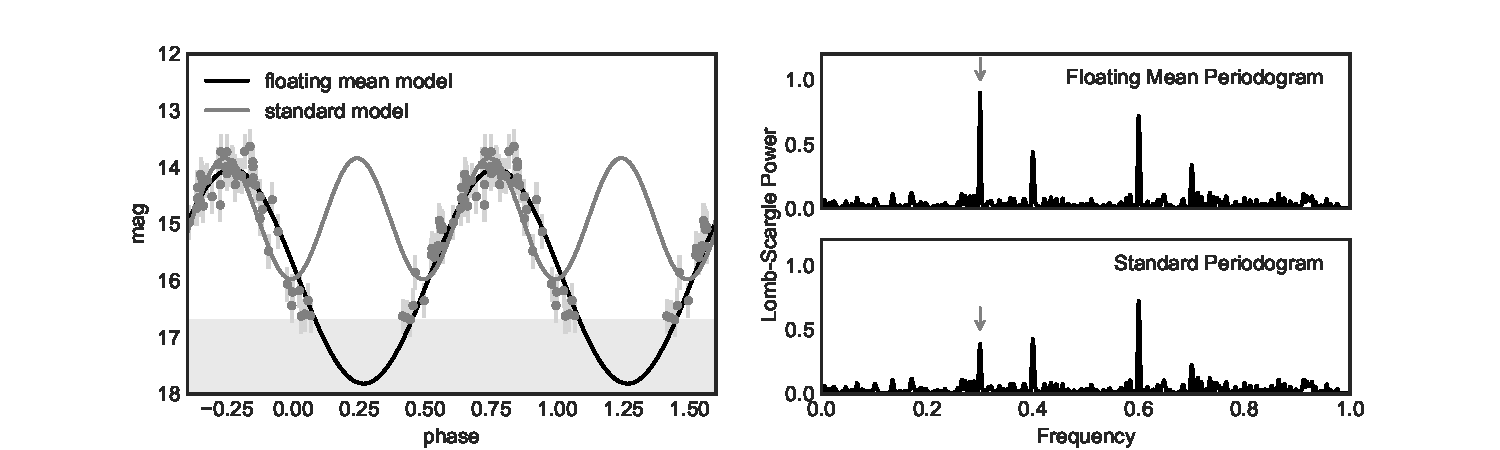
\includegraphics[width=\textwidth]{fig20_standard_vs_floatingmean}
  \caption{A comparison of the standard and floating mean periodograms for
    data with a frequency of 0.3 and a selection effect which removes
    faint observations.
    In this case the mean estimated from the observed data is not close to
    the true mean, which leads to the failure of the standard periodogram to
    recover the correct frequency. A floating mean model correctly recovers
    the true frequency of 0.3.
    \figlabel{standard-vs-floatingmean}}
\end{figure}

We have noted that the periodogram explored in \citep{Lomb76} and
\citep{Scargle82} is equivalent to computing the $\chi^2$ goodness-of-fit
of a sinusoid at each frequency.
Such a fit requires that the data be pre-centered; that is,
\begin{equation}
  \int_0^P g(t) dt = 0
\end{equation}fitting a sinusoid to the data at each
frrrequires the data to be pre-centered; i.e. the signal
must be modified so that 


will only work correctly if the data is pre-centered so
that a sinusoid with no offset will fit the data.
In the past this was primarily accomplished by pre-centering the data using the
mean estimated from the data points themselves.
With full phase coverage of the observed signal, this approach is generally
robust, but due to selection effects and survey cadence, full coverage can
not always be guaranteed.
This can potentially lead to situations where the periodogram entirely misses
peaks of interest; an example of this is shown in \fig{standard-vs-floatingmean}.
This simulates noisy observations of a sinusoidal signal situation in which the faintest parts of the light curve fall below the detection threshold.
Using the standard periodogram, where the mean is estimated from the observations, leads to a periodogram that misses the true period of 0.3 days.
The floating-mean periodogram, on the other hand, fits the mean as part of the model and more accurately characterizes the periodic content of the partially-observed data.

\subsection{Fitting Higher-order Models}

\citet{Bretthorst88}

\todo{Use a multi-band periodogram on Kepler Data}

\todo{Show poor performance on eclipsing data}


\section{Practical Considerations when using Lomb-Scargle Periodograms}
\sectlabel{practical-considerations}

\subsection{Choosing a Frequency Grid}
The choice of frequency grid for a Lomb-Scargle analysis is an important one
that is too-often glossed-over, probably because the choice is so
straightforward in the more familiar case of uniformly-sampled data.
For non-uniform data, it is not so simple, and there are two important
considerations: the {\bf frequency limits} and the {\bf grid spacing}.

The frequency limit on the low end is relatively easy: for a set of observations
spanning a length of time $T$,
a signal with frequency $1/T$ will complete exactly one oscillation cycle,
and so this is a suitable minimum frequency.
Often, it's more convenient just to set this minimum frequency to zero, as it
doesn't add much of a computational burden and is unlikely to add any
significant spurious peak to the periodogram.

The high-frequency limit is more interesting, and goes back to the discussion
of Nyquist and/or limiting frequencies from \sect{pseudo-nyquist}:
in order to not miss relevant information, it is important to compute the
periodogram up to some well-motivated limiting frequency $f_{max}$. This could
be a true Nyquist limit based on the \citep{Eyer99} definition, a pseudo-Nyquist
limit based on careful scrutiny of the window function (cf. \fig{kepler-data}),
or a limiting frequency based on the integration time of individual
observations.

\begin{figure}[ht]
  \centering
  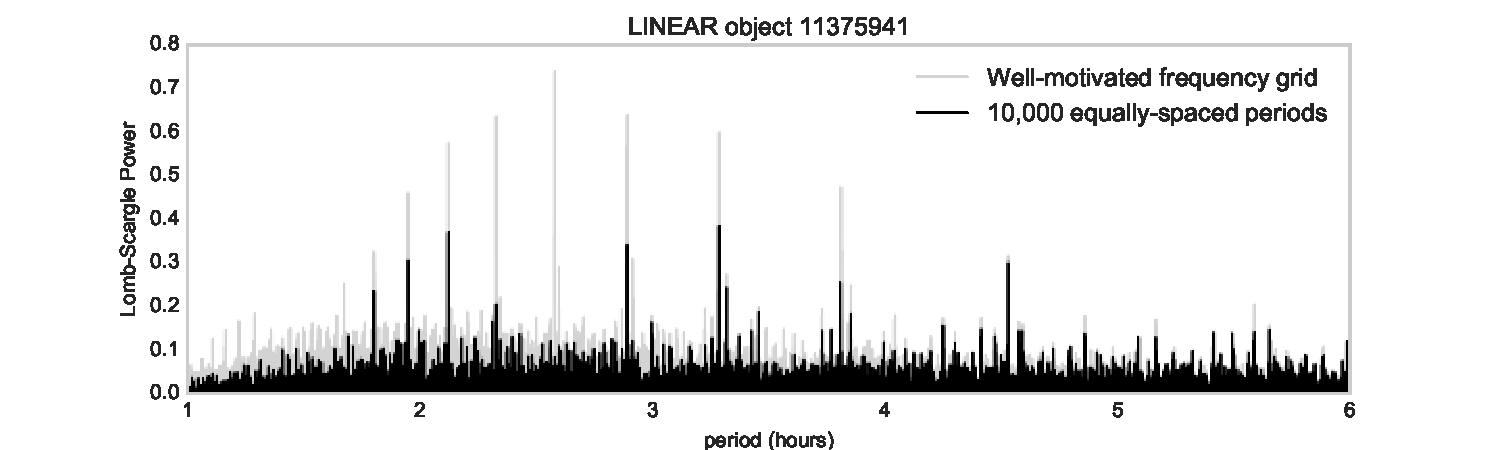
\includegraphics[width=\textwidth]{fig19_LINEAR_coarse_grid}
  \caption{An example of a poorly-chosen frequency grid for the data in
    \fig{LINEAR-data}. The dark curve shows a periodogram evaluated on a
    grid of 10,000 equally-spaced periods; the light curve shows the true
    periodogram (evaluated at ${\sim}200,000$ equally-spaced frequencies).
    This demonstrates that using too coarse a grid can lead to a periodogram
    that entirely misses relevant peaks.
    \figlabel{LINEAR-coarse-grid}}
\end{figure}

With the frequency range decided, we next must determine how finely to sample
the frequencies between the limits.
This turns out to be quite important: if you choose too fine a grid, it can
lead to unnecessarily long computation times that can add up quickly in the
case of large surveys. If you choose too coarse a grid, you
risk entirely missing narrow peaks that fall between grid points.
For example, \fig{LINEAR-coarse-grid} shows the true, well-sampled periodogram
(gray line), along with a periodogram computed for 10,000 equally-spaced
periods covering the same range (black line).
Because the spacing of the 10,000-point grid is much larger than the width of
the periodogram peaks, the computation {\it entirely misses} the most
important peaks in the periodogram!

This shows us that it's important to choose grid spacings smaller than the
expected widths of the periodogram peaks.
From our discussion of windowing in \sect{window-functions}
(particularly \fig{rectangular-window}), we know that data observed through a
rectangular window of length $T$ will have sinc-shaped peaks of width
${\sim}1/T$.
To ensure that our grid sufficiently covers each peak, it is prudent to
over-sample by some factor---say $n_{over}$ samples per peak---and
use a grid of size $\Delta f = \frac{1}{n_{over} T}$.
This pushes the total number of required periodogram evaluations to
\begin{equation}
  \eqlabel{n-eval}
  N_{eval} = n_o T f_{max}
\end{equation}

Depending on the characteristics of the dataset, this number can vary greatly.
For example, the Kepler data shown in \fig{kepler-data} has a pseudo-Nyquist
frequency of $48.9\ {\rm days}^{-1}$ and
an observing window of $T = 90\ {\rm days}$.
To compute five samples per peak thus requires $N_{eval} \approx 22,000$
evaluations of the periodogram.

On the other hand, the LINEAR data shown in \fig{LINEAR-data} does not have
any noteable aliasing structure in its window function.
In this case the maximum detectable frequency is the Nyquist limit defined
by its temporal resolution, which is 6 digits beyond the decimal point in days.
From \eq{nonuniform-nyquist}, we can write $f_{Ny} = 500,000\ {\rm days}^{-1}$.
Given the observing window of $T = 1962\ {\rm days}$, we find that five
evaluations per peak across the entire detectable frequency range
would require $N_{eval} \approx 4.9 \times 10^9$ evaluations of the periodogram!
Computing this large a periodogram in most cases is computationally intractable
(see \sect{algorithmic-considerations}), and so in practice one must choose
a smaller limiting frequency based on prior information about what kind of
signals are expected in the data: for example, in \fig{LINEAR-power}, we chose
a limiting frequency of $f_{max} = (1\ {\rm hour})^{-1}$ based on typical
oscillation periods of SX Phe-type stars. This leads to a much more manageable
$N_{eval} \approx 240,000$ periodogram evaluations.

By comparison, data from the upcoming LSST survey \citep{Ivezic08LSST}
will fall somewhere in-between: full frequency coverage of
the 10-year data up to a limiting frequency defined by the 30-second
exposure time for each observation will require roughly 2.5 million
periodogram evaluations per object, which for fast Lomb-Scargle implementations
(see the next section) can be accomplished in seconds on a single core.

One final note: although it can be more easily interpretable to
visualize periodograms as a function of period rather than a function of
frequency, the peak widths are not constant in period.
Thus regular period grids tend to over-sample at large periods and under-sample
at small periods;
for this reason it is preferable to use a regular grid in frequency.




\subsection{Algorithmic Considerations}
\sectlabel{algorithmic-considerations}
Given the size of the frequency grid required to fully characterize the periods
from a given dataset, it is vital to have an efficient algorithm for evaluating
the periodogram. Unfortunately, the periodogram itself is a relatively slow
operation.

Suppose you have a set of $N$ observations over a time-span $T$ for an average
cadence of $\overline{\delta t} = N/T$.
From \eq{n-eval} we see that the number of frequencies evaluated is
$N_f \propto T f_{max} = N f_{max} / \overline{\delta t}$.
Holding constant the average survey cadence $\overline{\delta t}$ and individual
observation properties (which control $f_{max}$), we find that the number of
frequencies is directly proportional to the number of data points.
The computation of the Lomb-scargle periodogram in \eq{lomb-scargle-periodogram}
requires sums over $N$ sinusoids at each of the
$N_f$ frequencies, and thus we see that the
na{\"i}ve scaling of the algorithm with the size of the dataset is
$\mathcal{O}(N^2)$, when survey properties are held constant.
Due to the trigonometric functions involved, this turns out to be a rather
``expensive'' $\mathcal{O}(N^2)$, which makes the straightforward
implementation impractical for even modestly-sized datasets.

Fortunately, several faster implementations have been proposed to compute the
periodogram to arbitrary precision in $\mathcal{O}(N\log N)$ time.
The first of these is discussed in \citet{Press89}, which uses an inverse
interpolation operation along with a Fast Fourier Transform to compute the
trigonometric components of \eq{lomb-scargle-periodogram} very efficiently over
a large number of frequencies.
A qualitatively similar approach is presented by \citet{Leroy2012},
and makes use of the Non-equispaced Fast Fourier Transform
\citep[NFFT, see][]{Keiner2009} to compute the Lomb-Scargle periodogram about
a factor of 10 faster than the \citet{Press89} approach.
All periodograms in this paper were computed using the Astropy
implementation of the \citet{Press89} algorithm, which was adapted from Python
code released to accompany \citet{VanderPlas2015}.


\subsection{Normalization of the Periodogram}

\begin{itemize}
  \item $\chi^2$ normalization
  \item PSD normalization
  \item Other normalizations \citep{Baluev2008}
\end{itemize}


\section{Uncertainties in Periods}
\sectlabel{uncertainties}

\begin{itemize}
  \item Peak Width and why it's a poor proxy
  \item False Alarm Probability and its pitfalls
  \item Baluev method and why it's not enough
  \item Motivation and example of Bootstrap
\end{itemize}


\section{Generalizations \& Challenges}
\sectlabel{generalizations}

\begin{itemize}
\item floating-mean
\item Uncertainties in Data
\item Bayesian view is (almost always) not useful
\item Multiterm makes the true period fit better, but also bumps the background noise.
\end{itemize}


\section{Conclusion and Summary}

(Summarize key recommendations here)

\bibliographystyle{apj}
\bibliography{PracticalLombScargle}


\end{document}
